% Options for packages loaded elsewhere
% Options for packages loaded elsewhere
\PassOptionsToPackage{unicode}{hyperref}
\PassOptionsToPackage{hyphens}{url}
\PassOptionsToPackage{dvipsnames,svgnames,x11names}{xcolor}
%
\documentclass[
  article,
  nofooter,
  noheadings]{jss}
\usepackage{xcolor}
\usepackage{amsmath,amssymb}
\setcounter{secnumdepth}{-\maxdimen} % remove section numbering
\usepackage{iftex}
\ifPDFTeX
  \usepackage[T1]{fontenc}
  \usepackage[utf8]{inputenc}
  \usepackage{textcomp} % provide euro and other symbols
\else % if luatex or xetex
  \usepackage{unicode-math} % this also loads fontspec
  \defaultfontfeatures{Scale=MatchLowercase}
  \defaultfontfeatures[\rmfamily]{Ligatures=TeX,Scale=1}
\fi
\usepackage{lmodern}
\ifPDFTeX\else
  % xetex/luatex font selection
\fi
% Use upquote if available, for straight quotes in verbatim environments
\IfFileExists{upquote.sty}{\usepackage{upquote}}{}
\IfFileExists{microtype.sty}{% use microtype if available
  \usepackage[]{microtype}
  \UseMicrotypeSet[protrusion]{basicmath} % disable protrusion for tt fonts
}{}
\makeatletter
\@ifundefined{KOMAClassName}{% if non-KOMA class
  \IfFileExists{parskip.sty}{%
    \usepackage{parskip}
  }{% else
    \setlength{\parindent}{0pt}
    \setlength{\parskip}{6pt plus 2pt minus 1pt}}
}{% if KOMA class
  \KOMAoptions{parskip=half}}
\makeatother
% Make \paragraph and \subparagraph free-standing
\makeatletter
\ifx\paragraph\undefined\else
  \let\oldparagraph\paragraph
  \renewcommand{\paragraph}{
    \@ifstar
      \xxxParagraphStar
      \xxxParagraphNoStar
  }
  \newcommand{\xxxParagraphStar}[1]{\oldparagraph*{#1}\mbox{}}
  \newcommand{\xxxParagraphNoStar}[1]{\oldparagraph{#1}\mbox{}}
\fi
\ifx\subparagraph\undefined\else
  \let\oldsubparagraph\subparagraph
  \renewcommand{\subparagraph}{
    \@ifstar
      \xxxSubParagraphStar
      \xxxSubParagraphNoStar
  }
  \newcommand{\xxxSubParagraphStar}[1]{\oldsubparagraph*{#1}\mbox{}}
  \newcommand{\xxxSubParagraphNoStar}[1]{\oldsubparagraph{#1}\mbox{}}
\fi
\makeatother


\usepackage{longtable,booktabs,array}
\usepackage{calc} % for calculating minipage widths
% Correct order of tables after \paragraph or \subparagraph
\usepackage{etoolbox}
\makeatletter
\patchcmd\longtable{\par}{\if@noskipsec\mbox{}\fi\par}{}{}
\makeatother
% Allow footnotes in longtable head/foot
\IfFileExists{footnotehyper.sty}{\usepackage{footnotehyper}}{\usepackage{footnote}}
\makesavenoteenv{longtable}
\usepackage{graphicx}
\makeatletter
\newsavebox\pandoc@box
\newcommand*\pandocbounded[1]{% scales image to fit in text height/width
  \sbox\pandoc@box{#1}%
  \Gscale@div\@tempa{\textheight}{\dimexpr\ht\pandoc@box+\dp\pandoc@box\relax}%
  \Gscale@div\@tempb{\linewidth}{\wd\pandoc@box}%
  \ifdim\@tempb\p@<\@tempa\p@\let\@tempa\@tempb\fi% select the smaller of both
  \ifdim\@tempa\p@<\p@\scalebox{\@tempa}{\usebox\pandoc@box}%
  \else\usebox{\pandoc@box}%
  \fi%
}
% Set default figure placement to htbp
\def\fps@figure{htbp}
\makeatother





\setlength{\emergencystretch}{3em} % prevent overfull lines

\providecommand{\tightlist}{%
  \setlength{\itemsep}{0pt}\setlength{\parskip}{0pt}}





\usepackage{orcidlink,thumbpdf,lmodern}

\newcommand{\class}[1]{`\code{#1}'}
\newcommand{\fct}[1]{\code{#1()}}
\makeatletter
\@ifpackageloaded{tcolorbox}{}{\usepackage[skins,breakable]{tcolorbox}}
\@ifpackageloaded{fontawesome5}{}{\usepackage{fontawesome5}}
\definecolor{quarto-callout-color}{HTML}{909090}
\definecolor{quarto-callout-note-color}{HTML}{0758E5}
\definecolor{quarto-callout-important-color}{HTML}{CC1914}
\definecolor{quarto-callout-warning-color}{HTML}{EB9113}
\definecolor{quarto-callout-tip-color}{HTML}{00A047}
\definecolor{quarto-callout-caution-color}{HTML}{FC5300}
\definecolor{quarto-callout-color-frame}{HTML}{acacac}
\definecolor{quarto-callout-note-color-frame}{HTML}{4582ec}
\definecolor{quarto-callout-important-color-frame}{HTML}{d9534f}
\definecolor{quarto-callout-warning-color-frame}{HTML}{f0ad4e}
\definecolor{quarto-callout-tip-color-frame}{HTML}{02b875}
\definecolor{quarto-callout-caution-color-frame}{HTML}{fd7e14}
\makeatother
\makeatletter
\@ifpackageloaded{caption}{}{\usepackage{caption}}
\AtBeginDocument{%
\ifdefined\contentsname
  \renewcommand*\contentsname{Table of contents}
\else
  \newcommand\contentsname{Table of contents}
\fi
\ifdefined\listfigurename
  \renewcommand*\listfigurename{List of Figures}
\else
  \newcommand\listfigurename{List of Figures}
\fi
\ifdefined\listtablename
  \renewcommand*\listtablename{List of Tables}
\else
  \newcommand\listtablename{List of Tables}
\fi
\ifdefined\figurename
  \renewcommand*\figurename{Figure}
\else
  \newcommand\figurename{Figure}
\fi
\ifdefined\tablename
  \renewcommand*\tablename{Table}
\else
  \newcommand\tablename{Table}
\fi
}
\@ifpackageloaded{float}{}{\usepackage{float}}
\floatstyle{ruled}
\@ifundefined{c@chapter}{\newfloat{codelisting}{h}{lop}}{\newfloat{codelisting}{h}{lop}[chapter]}
\floatname{codelisting}{Listing}
\newcommand*\listoflistings{\listof{codelisting}{List of Listings}}
\makeatother
\makeatletter
\makeatother
\makeatletter
\@ifpackageloaded{caption}{}{\usepackage{caption}}
\@ifpackageloaded{subcaption}{}{\usepackage{subcaption}}
\makeatother
\makeatletter
\@ifpackageloaded{tcolorbox}{}{\usepackage[skins,breakable]{tcolorbox}}
\makeatother
\makeatletter
\@ifundefined{shadecolor}{\definecolor{shadecolor}{rgb}{.97, .97, .97}}{}
\makeatother
\makeatletter
\makeatother
\makeatletter
\ifdefined\Shaded\renewenvironment{Shaded}{\begin{tcolorbox}[enhanced, boxrule=0pt, borderline west={3pt}{0pt}{shadecolor}, interior hidden, frame hidden, breakable, sharp corners]}{\end{tcolorbox}}\fi
\makeatother
\usepackage{bookmark}
\IfFileExists{xurl.sty}{\usepackage{xurl}}{} % add URL line breaks if available
\urlstyle{same}
\hypersetup{
  pdftitle={Caractérisation et évolution des précipitations extrêmes horaires en France à partir d'un modèle régional de climat à convection profonde résolue},
  pdfauthor={Nicolas Decoopman; Juliette Blanchet; Antoine Blanc},
  colorlinks=true,
  linkcolor={blue},
  filecolor={Maroon},
  citecolor={Blue},
  urlcolor={Blue},
  pdfcreator={LaTeX via pandoc}}


%% -- Article metainformation (author, title, ...) -----------------------------

%% Author information
\author{Nicolas Decoopman\\UGA M2 SSD \And Juliette Blanchet\\CNRS,
IGE \And Antoine Blanc\\RTM}
\Plainauthor{Nicolas Decoopman, Juliette Blanchet, Antoine
Blanc} %% comma-separated

\title{Caractérisation et évolution des précipitations extrêmes horaires
en France à partir d'un modèle régional de climat à convection profonde
résolue}
\Plaintitle{Caractérisation et évolution des précipitations extrêmes
horaires en France à partir d'un modèle régional de climat à convection
profonde résolue} %% without formatting

%% an abstract and keywords
\Abstract{Le changement climatique provoque un réchauffement global
(+1,1°C), plus marqué en France métropolitaine (+1,7°C) et dans les
Alpes françaises (+2°C) depuis l'ère préindustrielle. L'air plus chaud
contient davantage d'humidité, ce qui favorise théoriquement
l'augmentation des précipitations extrêmes, bien que les tendances
effectivement observées varient selon les régions et les circulations
atmosphériques. Les modèles climatiques classiques (GCM et RCM) sont
limités pour représenter les précipitations extrêmes à résolution
infra-journalière en raison de leur faible résolution et de la
paramétrisation de la convection. En effet, d'autres facteurs entrent en
jeu tel que l'évolution des circulations atmosphériques, la
disponibilité de l'humidité et les processus convectifs. Les modèles à
résolution spatiale (CP-RCM), comme CNRM-AROME (2,5 km), permettent
désormais une meilleure représentation explicite de la convection
profonde. Le stage vise à analyser les tendances des précipitations
extrêmes horaires en France (1959-2022) grâce aux données CP-RCM et
pluviométriques, en appliquant des modèles de valeurs extrêmes (GEV)
stationnaires et non stationnaires.}

%% at least one keyword must be supplied
\Keywords{Changement climatique, Précipitations
extrêmes, Clausius-Clapeyron, Convection profonde, Modèles climatiques
régionaux (RCM), Modèles de climat à résolution kilométrique
(CP-RCM), CNRM-AROME, Théorie des valeurs extrêmes (GEV), Tendances non
stationnaires}

%% publication information
%% NOTE: Typically, this can be left commented and will be filled out by the technical editor
%% \Volume{50}
%% \Issue{9}
%% \Month{June}
%% \Year{2012}
%% \Submitdate{2012-06-04}
%% \Acceptdate{2012-06-04}
%% \setcounter{page}{1}
%% \Pages{1--xx}

%% The address of (at least) one author should be given
%% in the following format:
\Address{
Nicolas Decoopman\\
\\~
Juliette Blanchet\\
\\~
Antoine Blanc\\
\\~

}

\begin{document}
\maketitle


\newpage

\section{Introduction et contexte}\label{introduction-et-contexte}

Le changement climatique entraine un réchauffement de l'air à la surface
de la planète, plus marqué sur les continents que sur les océans
\citep{IPCC2021}. L'augmentation est de +1°C à l'échelle mondiale,
+1,7°C à l'échelle de la France métropolitaine et +2°C à l'échelle des
Alpes françaises depuis l'ère préindustrielle. Par ailleurs, la relation
de Clausius-Clapeyron montre que l'air chaud contient plus d'humidité
(+7\%/°C) \citep{clapeyron1834}. Autrement dit, à +1°C, une même masse
d'air pourra contenir 7\% de vapeur d'eau en plus. Du fait de la poussée
d'Archimède, l'air chaud entourée d'air plus froid aura tendance à
monter. L'ascension de l'air chaud dans l'atmosphère entraîne son
refroidissement adiabatique, provoquant la condensation de la vapeur
d'eau qui se transforme en précipitations \citep{meteofrance}.
Toutefois, en conditions calmes le noyau de la distribution des
précipitations n'exploite pas pleinement ce surplus d'humidité. Il
existe des contraintes énergétiques (bilan radiatif, évaporation,
échanges océan‑air) et dynamiques (subsidence, vent synoptique) qui
limitent l'augmentation des précipitations moyennes à seulement
1--3\%/°C \citep{IPCC2021}. En revanche, lors d'événements convectifs
intenses (orage, cyclogenèse rapide) l'ascension rapide condense presque
intégralement ce surplus, et les pluies maximales sur des durées courtes
augmentent de 5 à 8\,\% par °C, soit presque au même rythme que le
potentiel théorique. Les extrêmes de précipitation suivent de près la
loi de Clausius--Clapeyron, tandis que la pluie moyenne reste sous
l'influence de nombreux autres facteurs énergétiques et dynamiques
\citep{ogorman2015contrasting}. Ainsi, en réponse au réchauffement
climatique il existe une augmentation \emph{théorique} des
précipitations extrêmes. Cette augmentation est variable suivant les
changements de circulations atmosphériques et peut être amplifiée
localement \citep{blanchet2021explaining}.

Les précipitations extrêmes sont définies comme des épisodes de fortes
pluies intenses sur de courtes durées (1h à 24h) et correspondent à la
queue de la distribution des intensités pluviométriques. Ils sont au
coeur des préoccupations climatiques et sociétales. Ces épisodent
provoquent 90\% des coûts liés aux inondations, aux glissements de
terrain et aux ruptures d'infrastructures \citep{IPCC_2022_WGIII}. En
2024, de nombreux événements de ce type ont fait l'actualité, par
exemple en Espagne orientale, au Népal, en Afghanistan ou en Europe
centrale \citep{WMO2025}. En particulier en France, en juin 2024, des
pluies intenses en haute altitude qui ont contribué à des inondations
majeures dans le massif des Écrins \citep{Blanc2024} ; en octobre, plus
de 600 mm en 48h dans le département de l'Ardèche
\citep{MeteoFrance2024_episodesArdeches} ; en mai 2025, des orages
courts mais extrêmement intenses (localement dépassant 120 mm/h) ont
causé des dommages généralisés dans le sud du département du Var
\citep{MeteoFrance2025}.

La fréquence et l'intensité des pluies extrêmes journalières ont
augmenté depuis les années\,1950. Le nombre annuel de jours à plus\,de
10\,mm/j de précipitation a augmenté au niveau mondial de +0,2 à
+0,3\,jour par décennie sur 1951--2010 \citep{Donat2013} avec 29\% des
mailles terrestres présentant une hausse significative. 71\% des régions
terrestres montrent une hausse significative de l'intensité des
précipitations maximales \citep{IPCC2021}. Les événements de type
``pluie extrême journalières avec retour statistique décennal'' ont
augmenté +6,7\%. Dans le sud‑est de la France, la fréquence des épisodes
méditerranéens extrêmes (cumuls\,\textgreater\,200\,mm en 24h) a doublé
entre 1961 et 2020, même si la variabilité interannuelle reste très
forte \citep{meteofrance2024_episodesMediterraneens} et l'intensité
moyenne des extrêmes journaliers a augmenté de +22\% entre 1961 et 2015
\citep{Ribes2019}. La tendance des maxima annuels de précipitations
quotidiennes était inexistante jusqu'aux années 1990 et d'environ +20 à
+40\% depuis. La hausse du niveau de précipitations journalières
attendue en moyenne tous les 20 ans en automne pourrait atteindre un
ordre de grandeur d'environ 100\,\% de sa valeur moyenne
\citep{blanchet2021explaining}. En France, un scénario de réchauffement
de +4\,°C conduirait à +15\% d'augmentation des pluies extrêmes
journalières en moyenne et jusqu'à +20\% dans la moitié nord du pays
\citep{soubeyroux:hal-04991790}.

Les extrêmes horaires, mesurés sur des pas de temps de 1h ou moins, sont
essentiels pour caractériser les phénomènes convectifs intenses (averses
orageuses, orages stationnaires) souvent responsables d'inondations
flash. Faute de séries longues et spatialisées, il n'existe pas
d'analyse systématique des tendances sub‑journalières à l'échelle
globale\,; les données sont souvent éparses et de courte durée. Malgré
cela, plusieurs études régionales détectent une intensification des
extrêmes horaires sur presque tous les continents, mais la confiance
dans une hausse globale reste très faible \citep{IPCC2021}. Un
accroissement des pluies extrêmes est relevée aux États-Unis, en Chine
(l'été), en Australie\,(sur l'année), en Afrique du Sud (l'été), en
Inde, en Malaisie, et en Italie. Plusieurs travaux mettent en évidence,
selon la méthode et la région considérées, des sensibilités de l'ordre
de +7\% à +14\% par °C, c'est‑à‑dire jusqu'à deux fois la pente de
Clausius‑Clapeyron. En France, peu d'études régionales caractérisent
explicitement cette hausse des cumuls extrêmes. Les valeurs maximales
observées sur 1h atteignent maintenant 40--60\,mm dans les événements
méditerranéens majeurs, contre 30--40\,mm dans les années 1980--1990
\citep{meteofrance2024_episodesMediterraneens}. Seul l'étude de
\citet{Berghald2025} semble chiffrer l'évolution des tendances des
extrêmes horaires dans les Alpes : +100\% en novembre entre 1990 et 2020
du niveau de précipitation attendu en moyenne une fois tous les 20 ans.
Les tendances annuelles horaires sont majoritairement non
significatives\,et montrent plutôt un gradient est--ouest (positives sur
les Hautes-Alpes, négatives sur les pré‑Alpes).

Il n'existe pas de définition consensuelle de ce qui caractérise un
\emph{extrême}. Certains auteurs étudient des précipitations
d'intensités au-dessus du 99e percentile ou des maxima
saisonniers/annuels. D'autres, cependant, considèrent les précipitations
extrêmes comme des événements qui sont rarement ou jamais rencontrés
dans la vie d'un humain (par exemple, des niveaux de précipitations aux
quels on s'attend une fois tous les 10, 20 ou 50 ans). Dans le présent
article, nous nous intéressons principalement à la deuxième classe, car
ces événements sont susceptibles de produire les impacts les plus forts.
Plus précisément, nous définissons ici les extrêmes comme des niveaux de
retour de 10 ans.

Dans les années 1990, la numérisation des observations continues
(notamment par Électricité de France, une entreprise électrique
française, ainsi que par diverses autres institutions) a fourni un accès
à 30-40 ans de données pour environ soixante stations, permettant la
caractérisation des précipitations extrêmes à des échelles de temps
infra-journalières \citep{Garcon1993}.

Dans l'objectif de dégager des tendances durables (changement
climatique) en opposition aux variations naturelles (variabilité
climatique), il convient d'utiliser des données issues de modèles de
climat sur de longues périodes. Ces dernières années, l'utilisation des
modèles régionaux de climat à haute résolution (CP-RCM pour
Convection-Permitting Regional Climate Models, avec une résolution de 1
à 3 km) a marqué une avancée significative. Ces modèles simulent
explicitement la convection profonde, ce qui leur permet de capturer des
échelles spatio-temporelles plus fines. Cette approche ouvre de
nouvelles perspectives prometteuses pour l'analyse climatique
\citep{prein2015regional}.

L'objectif de cette étude est de caractériser et d'étudier les tendances
de précipitations extrêmes horaires en France. Les précipitations
extrêmes sont définies par leur caractère exceptionnel au regard de la
climatologie locale. Une méthode courante consiste à considérer les
maxima pour une période et un pas de temps donnés
\citep{blanchet2022instrumental}.

\section{Méthodologie}\label{muxe9thodologie}

\subsection{Données utilisées}\label{donnuxe9es-utilisuxe9es}

Dans cette étude, le modèle numérique Application of Research to
Operations at MEsoscale (AROME) a été choisi
\citep{caillaud2021simulation}. C'est un modèle CP-RCM de résolution
spatiale 2,5 km et temporelle 1h, forcé par réanalyse ERA5
\citep{hersbach2020era5} offrant des données de précipitations de 1959 à
2022. En parallèle, l'étude utilise aussi les données de précipitations
issues d'observation Météo-France \citep{meteofrance2024} au pas de
temps journalier (1959-2022) et horaire (1990-2022).

\subsection{Statistiques descriptives}\label{statistiques-descriptives}

Par extraction, transformation et chargement, les statistiques
descriptives suivantes sont générées : nombre de jour de pluie (seuil
fixé à 1mm/j), cumul de précipitations, maximum de précipitations. Ceci
en chaque point de grille AROME et chaque station Météo-France à partir
des données journalières de 1959 à 2022 et 1990 à 2022 ; et des données
horaires de 1990 à 2022, pour chaque année et chaque saison (ou mois).

Les saisons sont définies par \textbf{SON} pour septembre (\textbf{SEP})
octobre (\textbf{OCT}) novembre (\textbf{NOV}), \textbf{DJF} pour
décembre (\textbf{DEC}) janvier (\textbf{JAN}) février (\textbf{FEV}),
\textbf{MAM} pour mars (\textbf{MAR}) avril (\textbf{AVR}) mai
(\textbf{MAI}), et \textbf{JJA} pour juin (\textbf{JUI}) juillet
(\textbf{JUILL}) août (\textbf{AOU}). L'année hydrologique
(\textbf{HYDRO}) est définie comme la période allant du 1er septembre de
l'année N au 31 août de l'année N+1.

\subsection{Filtrage des séries}\label{filtrage-des-suxe9ries}

Pour chaque point géographique, chaque saison (ou mois) et chaque année,
on calcul la part de données manquantes dans la série temporelle. On
élimine toutes les années dont cette part dépasse le seuil fixé de 10\%.
On déduit le nombre d'années valides restantes. On ne garde que les
points géographiques qui possèdent au moins le nombre minimal d'années
exigé (50 ans pour les données journalières 1959-2022 et 25 ans pour les
données journalières 1990-2022 et les données horaires 1990-2022). Les
analyses suivantes ne portent plus que sur ce sous‑ensemble de stations
et d'années : on travaille ainsi avec des séries suffisamment complètes
et longues pour être fiables.

\subsection{Modélisation statistique}\label{moduxe9lisation-statistique}

\subsubsection{Définitions}\label{duxe9finitions}

Si on note \(x\) une réalisation de la variable aléatoire \(X\),
représentant le maximum annuel de précipitations en un point spatial
donné, alors la loi GEV (loi des valeurs extrêmes généralisée) est une
loi de probabilité continue paramétrée par le triplet
\(\theta = (\mu, \sigma, \xi)\) --- respectivement la position,
l'échelle (strictement positive) et la forme dont la fonction de
répartition cumulative (CDF) de la GEV est définie comme suit :

\[
F(x;\mu ,\sigma ,\xi ) = \exp \left\{ -\left[ 1 + \xi \left( \frac{x - \mu}{\sigma} \right) \right]^{-\frac{1}{\xi}} \right\}
\]

\subsubsection{Covariable temporelle}\label{covariable-temporelle}

On dispose d'une série temporelle de \(n\) maximas annuels indépendants
de précipitations pour un point géographique. Ces observations sont
notées \(\{x_1, x_2, \dots, x_n\}\) où chaque \(x_i\) est un maximum
annuel de précipitations observé à l'année \(t_i\) et qui suit une loi
GEV de paramètre \(\theta\). On transforme l'année \(t_i\) en une
covariable normalisée notée \(\tilde{t}_i\). Cette transformation est
simplement réalisée pour des raisons numériques mais elle ne change rien
au résultat théorique.

\[
\tilde{t}_i = \frac{t_i - t_{\min}}{t_{\max} - t_{\min}} \quad \text{avec} \quad \begin{cases}
t_{min} = \min_i t_i \\
t_{max} = \max_i t_i
\end{cases}
\]

On crée également une covariable temporelle avec point de rupture noté
\(t_+\) tel que :

\[
\tilde{t}_{i}^\ast =
\begin{cases}
0 & \text{si } t_i < t_+ \\
\displaystyle \frac{t_i - t_+}{t_{\max} - t_+} & \text{si } t_i \ge t_+
\end{cases}
\]

Ce codage permet d'appliquer une pente temporelle seulement après la
date de rupture, avec une covariable encore normalisée sur \([0,1]\)
dans la portion post-rupture.

\subsubsection{Modèles utilisés}\label{moduxe8les-utilisuxe9s}

Soit la covariable
\(t \in \mathbb{N} \mid t_{\min} \leq t \leq t_{\max}\). Le
\textbf{modèle stationnaire} est défini par :

\[
M_0(\theta_0) \quad \text{et} \quad \theta_0 = (\mu_0, \sigma_0, \xi_0) \quad
\begin{cases}
\mu(t) = \mu_0 \\
\sigma(t) = \sigma_0 \\
\xi(t) = \xi_0
\end{cases}
\]

Les \textbf{modèles non stationnaires} sont définis par :

\[
M_1(\theta_1) \quad \text{et} \quad \theta_1 = (\mu_0, \mu_1, \sigma_0, \xi_0) \quad
\begin{cases}
\mu(t) = \mu_0 + \mu_1 \cdot t \\
\sigma(t) = \sigma_0 \\
\xi(t) = \xi_0
\end{cases}
\]

\[
M_2(\theta_2) \quad \text{et} \quad \theta_2 = (\mu_0, \sigma_0, \sigma_1, \xi_0)
\quad
\begin{cases}
\mu(t) = \mu_0 \\
\sigma(t) = \sigma_0 + \sigma_1 \cdot t \\
\xi(t) = \xi_0
\end{cases}
\]

\[
M_3(\theta_3) \quad \text{et} \quad \theta_3 = (\mu_0, \mu_1, \sigma_0, \sigma_1, \xi_0)
\quad
\begin{cases}
\mu(t) = \mu_0 + \mu_1 \cdot t\\
\sigma(t) = \sigma_0 + \sigma_1 \cdot t \\
\xi(t) = \xi_0
\end{cases}
\]

Lorsqu'un point de rupture noté \(t_+\) est introduit, on note :

\[
t^\ast = t \cdot \mathbb{1}_{t > t_+} \quad \text{avec} \quad t_+ \in \mathbb{N}
\]

Les modèles \(M_1\), \(M_2\) et \(M_3\) deviennent respectivements
\(M_1^\ast\), \(M_2^\ast\) et \(M_3^\ast\). Sur cete même notation
\(\theta_i\) devient \(\theta^\ast_i\) avec \(i \in \{1, 2, 3\}\). Dans
cette étude, on réalise les modélisations stationnaire et
non-stationnaires avec pour covariable l'année et un effet temporel sur
\(\mu\) ou \(\sigma\) ou \(\mu\) et \(\sigma\). \(\xi\) est choisi comme
constant. Sur la base bibliographique, on choisi \(t_+ = 1985\)
\citep{blanchet2022instrumental}.

\subsubsection{Niveau de retour}\label{niveau-de-retour}

Le niveau de retour (ou quantile d'ordre \(1 - \tfrac{1}{T}\)) dans une
loi GEV correspond à une valeur seuil \(z_T\) que l'on dépasse, en
moyenne, une fois tous les \(T\) ans. Soit
\(X \sim \mathrm{GEV}(\mu, \sigma, \xi)\), alors en notant \(F^{-1}\) la
fonction quantile de la GEV, on obtient :

\begin{tcolorbox}[enhanced jigsaw, arc=.35mm, left=2mm, rightrule=.15mm, breakable, colframe=quarto-callout-color-frame, colback=white, bottomrule=.15mm, opacityback=0, leftrule=.75mm, toprule=.15mm]

\[
\mathbb{P}(X > z_T) = \frac{1}{T}, \quad \text{soit} \quad z_T = F^{-1}\left(1 - \frac{1}{T} \right) = 
\begin{cases}
\mu + \frac{\sigma}{\xi} \left[ \left( -\log\left(1 - \frac{1}{T}\right) \right)^{-\xi} - 1 \right] & \text{si } \xi \ne 0 \\
\mu - \sigma \log \left( -\log\left(1 - \frac{1}{T} \right) \right) & \text{si } \xi = 0 \quad \text{(Gumbel)}
\end{cases}
\]

\end{tcolorbox}

\subsubsection{Vraisemblance et maximum de
vraisemblance}\label{vraisemblance-et-maximum-de-vraisemblance}

Soit la fonction de vraisemblance
\({\displaystyle {\mathcal {L}}(\theta ;x)} : {\displaystyle \theta \mapsto f(x;\theta )}\).
La log-vraisemblance \(\ell(\theta) = \log \mathcal{L}(\theta)\) s'écrit
après développement (Annexes 1-1) :

\begin{tcolorbox}[enhanced jigsaw, arc=.35mm, left=2mm, rightrule=.15mm, breakable, colframe=quarto-callout-color-frame, colback=white, bottomrule=.15mm, opacityback=0, leftrule=.75mm, toprule=.15mm]

\[
\ell(\theta)=
-\sum_{i=1}^n\Bigl[
\log\sigma
+\Bigl(1+\tfrac1{\xi}\Bigr)\log z_i
+z_i^{-\frac{1}{\xi}}
\Bigr]
\quad \text{avec} \quad  z_i(\theta)=1+\xi\;\frac{x_i-\mu}{\sigma}
\tag{1}
\]

\end{tcolorbox}

On obtient alors :

\[
\scalebox{0.7}{
\(
\begin{aligned}
\ell_{M_0}(\mu_0, \sigma_0, \xi_0) &=
-\sum_{i=1}^n \left[
\log \sigma_0 +
\left(1 + \frac{1}{\xi_0} \right) \log \left(1 + \xi_0 \frac{x_i - \mu_0}{\sigma_0} \right) +
\left(1 + \xi_0 \frac{x_i - \mu_0}{\sigma_0} \right)^{-1/\xi_0}
\right]\\ 
\ell_{M_1}(\mu_0, \mu_1, \sigma_0, \xi_0) &=
-\sum_{i=1}^n \left[
\log \sigma_0 +
\left(1 + \frac{1}{\xi_0} \right) \log \left(1 + \xi_0 \frac{x_i - (\mu_0 + \mu_1 \cdot \tilde{t}_i)}{\sigma_0} \right) +
\left(1 + \xi_0 \frac{x_i - (\mu_0 + \mu_1 \cdot \tilde{t}_i)}{\sigma_0} \right)^{-1/\xi_0}
\right]\\ 
\ell_{M_2}(\mu_0, \sigma_0, \sigma_1, \xi_0) &=
-\sum_{i=1}^n \left[
\log (\sigma_0 + \sigma_1 \tilde{t}_i) +
\left(1 + \frac{1}{\xi_0} \right) \log \left(1 + \xi_0 \frac{x_i - \mu_0}{\sigma_0 + \sigma_1 \tilde{t}_i} \right) +
\left(1 + \xi_0 \frac{x_i - \mu_0}{\sigma_0 + \sigma_1 \tilde{t}_i} \right)^{-1/\xi_0}
\right]\\ 
\ell_{M_3}(\mu_0, \mu_1, \sigma_0, \sigma_1, \xi_0) &=
-\sum_{i=1}^n \left[
\log (\sigma_0 + \sigma_1 \tilde{t}_i) +
\left(1 + \frac{1}{\xi_0} \right) \log \left(1 + \xi_0 \frac{x_i - (\mu_0 + \mu_1 \tilde{t}_i)}{\sigma_0 + \sigma_1 \tilde{t}_i} \right) +
\left(1 + \xi_0 \frac{x_i - (\mu_0 + \mu_1 \tilde{t}_i)}{\sigma_0 + \sigma_1 \tilde{t}_i} \right)^{-1/\xi_0}
\right]
\end{aligned}
\tag{1'}
\)
}
\]

Les vraisemblances de \(M_1^*, M_2^*, M_3^*\) sont obtenues en
remplaçant \(\tilde{t}_i\) par \(\tilde{t}_i^\ast\) dans les expressions
ci-dessus.

En pratique, les paramètres \((\mu, \sigma, \xi)\) sont inconnus et
estimés à partir des données par un estimateur
\(\hat{\theta} = (\hat{\mu}, \hat{\sigma}, \hat{\xi})\) obtenu par
maximum de vraisemblance (MLE) via une optimisation numérique tel que
\(\hat{\theta} = \arg\max_{\theta} \, \ell(\theta)\). Il n'existe pas de
formule explicite des paramètres.

L'estimateur du niveau de retour \(\hat{z}_T\) s'écrit alors
\(\hat{z}_{T}\;=\;F^{-1}_{\hat{\theta}}\!\left(1-\frac{1}{T}\right)\).
Le MLE classique donne un point estimé, mais pas d'intervalle. On
souhaite aussi connaître l'incertitude autour de l'estimation de
\(\hat{z}_T\). Pour cela, on utilise la vraisemblance profilée.

\subsubsection{Vraisemblance profilée et intervalle de
confiance}\label{vraisemblance-profiluxe9e-et-intervalle-de-confiance}

\(z_T\) peut se réecrire sous la forme
\(\mu = z_T - \dfrac{\sigma}{\xi} \left[ \left( -\log\left(1 - \frac{1}{T} \right) \right)^{-\xi} - 1 \right]\).
La combinaison des paramètres temporels de la loi GEV conduit à une
expression linéaire en \(t\) :

\[
z_T(t) = z_{T,0} + z_{T,1} \cdot t
\]

En développant les paramètres soumis à un effet temporel et on
regroupant terme à terme on peut montrer que (Annexes 1-2) :

\[
\begin{aligned}
\mu_1(z_{T,1}) &= z_{T,1} -\dfrac{\hat{\sigma_1}}{\hat{\xi}_0}\Bigl(\bigl[-\log(1-\tfrac1T)\bigr]^{-\hat{\xi}_0}-1\Bigr)\\
\sigma_1(z_{T,1}) &= \dfrac{\hat{\xi}_0\,\bigl(z_{T,1}-\hat{\mu_1}\bigr)}{\bigl[-\log\!\bigl(1-\tfrac1T\bigr)\bigr]^{-\hat{\xi}_0}-1}\\
\end{aligned}
\]

On cherche l'intervalle de confiance sur \(z_{T,1}\) donc pour chaque
valeur candidate \(z_{T,1}\) dans une grille (autour de l'estimateur
\(\hat{z}_{T,1}\)), on maximise les log-vraisemblances
\textbf{\(\text{(1$'$)}\)} qui deviennent des log-vraisemblances
profilées \(\ell^{\,p}\) :

\[
\scalebox{0.7}{
\(
\begin{aligned}
\underset{\hat{\sigma}_1 = 0}{\ell_{M_1}^{\,p}(z_{T,1} \ ; \hat{\mu}_0, \hat{\sigma}_0, \hat{\xi}_0)} &= 
-\sum_{i=1}^n \left[
\log \hat{\sigma}_0 +
\left(1 + \frac{1}{\hat{\xi}_0} \right) \log \left(1 + \hat{\xi}_0 \frac{x_i - (\hat{\mu}_0 + \mu_1(z_{T,1}) \cdot \tilde{t}_i)}{\hat{\sigma}_0} \right) +
\left(1 + \hat{\xi}_0 \frac{x_i - (\hat{\mu}_0 + \mu_1(z_{T,1}) \cdot \tilde{t}_i)}{\hat{\sigma}_0} \right)^{-1/\hat{\xi}_0}
\right]\\
\underset{\hat{\mu}_1 = 0}{\ell_{M_2}^{\,p}(z_{T,1} \ ; \hat{\mu}_0, \hat{\sigma}_0, \hat{\xi}_0)} &= 
-\sum_{i=1}^n \left[
\log (\hat{\sigma}_0 + \sigma_1(z_{T,1}) \cdot \tilde{t}_i) +
\left(1 + \frac{1}{\hat{\xi}_0} \right) \log \left(1 + \hat{\xi}_0 \frac{x_i - \hat{\mu}_0}{\hat{\sigma}_0 + \sigma_1(z_{T,1}) \cdot \tilde{t}_i} \right) +
\left(1 + \hat{\xi}_0 \frac{x_i - \hat{\mu}_0}{\hat{\sigma}_0 + \sigma_1(z_{T,1}) \cdot \tilde{t}_i} \right)^{-1/\hat{\xi}_0}
\right]\\
\ell_{M_3}^{\,p}(z_{T,1} \ ; \hat{\mu}_0, \hat{\sigma}_0, \hat{\sigma}_1, \hat{\xi}_0) &= 
-\sum_{i=1}^n \left[
\log (\hat{\sigma}_0 + \hat{\sigma}_1 \tilde{t}_i) +
\left(1 + \frac{1}{\hat{\xi}_0} \right) \log \left(1 + \hat{\xi}_0 \frac{x_i - (\hat{\mu}_0 + \mu_1(z_{T,1}) \tilde{t}_i)}{\hat{\sigma}_0 + \hat{\sigma}_1 \tilde{t}_i} \right) +
\left(1 + \hat{\xi}_0 \frac{x_i - (\hat{\mu}_0 + \mu_1(z_{T,1}) \tilde{t}_i)}{\hat{\sigma}_0 + \hat{\sigma}_1 \tilde{t}_i} \right)^{-1/\hat{\xi}_0}
\right]\\
\end{aligned}
\tag{2}
\)
}
\]

On cherche donc :

\[
\hat{z}_{T,1} = \underset{z_{T,1}}{\arg\max} \; \ell_{M_\bullet}^{\,p}(z_{T,1} \ ; \hat{\theta}_{\bullet}) \quad \text{avec} \quad
\hat{\theta}_{\bullet} = \begin{cases}
\hat{\theta}_{1}^{\,p} = (\hat{\mu_0}, \hat{\sigma_0}, \hat{\xi_0}) & \text{pour } M_1 \\
\hat{\theta}_2^{\,p} = (\hat{\mu_0}, \hat{\sigma_0}, \hat{\xi_0}) & \text{pour } M_2 \\
\hat{\theta}_3^{\,p} = (\hat{\mu_0}, \hat{\sigma_0}, \hat{\sigma_1}, \hat{\xi_0}) & \text{pour } M_3 \\
\end{cases}
\]

On trace ainsi pour chaque modèle \(M_\bullet\) la fonction
\({\displaystyle \mathcal{L}_{M_\bullet} : z_{T,1} {\mapsto} \ell_{M_\bullet}^{\,p}(z_{T,1} \ ; \hat{\theta}_{\bullet})}\)

L'intervalle de confiance de \(\hat{z}_{T,1}\) pour un modèle
\(M_\bullet\) au seuil \((1 - \alpha)\) basé sur le profil de
vraisemblance est donné par :

\[
\operatorname{IC}_{M_\bullet}^{(1-\alpha)}\!\bigl(\hat{z}_{T,1}\bigr)
   = \Bigl\{\, z_{T,1}\;:\;
        2\bigl[\ell_{M_\bullet}^{\,p}(\hat{z}_{T,1} \ ; \hat{\theta}_{\bullet})-\ell_{M_\bullet}^{\,p}(z_{T,1} \ ; \hat{\theta}_{\bullet})\bigr]
        \le \chi^{2}_{1,\,1-\alpha} \Bigr\}
\]

où \(\chi^2_{1,1-\alpha}\) est le quantile d'ordre \(1 - \alpha\) d'une
loi du \(\chi^2\) à un degré de liberté. On fixe ici \(\alpha=0{,}10\).
Lorsque l'intervalle de confiance ne contient pas 0 alors
\(\hat{z}_{T,1}\) est significatif.

\subsection{Choix du meilleur modèle}\label{choix-du-meilleur-moduxe8le}

\subsubsection{Test du rapport de vraisemblance
(LRT)}\label{test-du-rapport-de-vraisemblance-lrt}

En tout point géographique on dispose de
\(M_0, M_1, M_2, M_3, M_1^\ast, M_2^\ast \text{ et } M_3^\ast\). Notons
\(k_j\) le nombre de paramètres du modèle \(M_j\). Pour chaque modèle
non stationnaire \(j\neq 0\) et chaque point \(i\)\,:

\[
\Lambda_{ij}=2\bigl(\ell_{ij}-\ell_{i0}\bigr)
\overset{H_0}{\sim}\chi^{2}_{\;k_j-k_0}.
\]

La \(p\)-valeur est
\(p_{ij}= \mathbb{P}(\chi^{2}_{k_j-k_0}\ge \Lambda_{ij}\bigr)\).

\subsubsection{Règle hiérarchique de
sélection}\label{ruxe8gle-hiuxe9rarchique-de-suxe9lection}

Soit \(\alpha=0{,}10\) le seuil d'intérêt. Si un des deux modèles
\(M_3\) ou \(M_3^\ast\) vérifie \(p_{ij}\le\alpha\), on retient
\(j=\arg\min_{j\in\{3,3^\ast\}} p_{ij}\). Sinon, on compare l'ensemble
des six modèles non stationnaires et l'on sélectionne
\(j=\arg\min_{j\in\{1,1^\ast,2,2^\ast,3,3^\ast\}} p_{ij}\). Cette double
étape privilégie les formes \emph{simultanément} temporelles sur \(\mu\)
et \(\sigma\) quand elles sont statistiquement justifiées. Cela assure
que la complexité n'est introduite que lorsqu'elle apporte une
information statistiquement crédible tout en livrant, pour chaque poste,
un modèle non stationnaire.

\subsection{Calcul des tendances}\label{calcul-des-tendances}

A partir des niveaux de retour 10 ans (\(T = 10\)) la tendance relative
(en \%) est calculée via la formule ci-dessous. Un exemple de calcul est
disponible en annexes 2-6.

\begin{tcolorbox}[enhanced jigsaw, arc=.35mm, left=2mm, rightrule=.15mm, breakable, colframe=quarto-callout-color-frame, colback=white, bottomrule=.15mm, opacityback=0, leftrule=.75mm, toprule=.15mm]

\[
\text{Tendance} = \frac{z_T^{2022} - z_T^{1995}}{z_T^{1995}} \cdot {100}
\]

\end{tcolorbox}

\subsection{Concordance}\label{concordance}

On évalue l'accord entre les statistiques descriptives et les tendances
obtenues à partir des simulations du modèle AROME et celles observées
dans la réalité. Pour ce faire, chaque station Météo-France est associée
au point de grille AROME (2,5 km × 2,5 km) correspondant à sa
localisation géographique. Cette correspondance permet de calculer la
corrélation de Pearson (\emph{r}) ainsi que l'erreur moyenne (\emph{ME})
entre les valeurs observées et simulées.

\subsection{Représentation
cartographique}\label{repruxe9sentation-cartographique}

Pour homogénéiser les amplitudes extrêmes entre jeux de données (AROME
et données observées), on applique une saturation de couleur suivant la
période étudiée. Soit une période
\(P \in \{\text{HYDRO}, \text{DJF},\text{MAM},\text{JJA},\text{SON}\}\)
ou
\(P \in \{\text{JAN},\text{FEV},\text{MAR},\text{...},\text{OCT},\text{NOV},\text{DEC}\}\).
Pour chaque données (nombre de jour de pluie, cumul, moyenne des maxima,
tendance relative) \(T_j\) avec \(j \in P\), on calcule le \emph{p}-ième
percentile des valeurs absolues :

\[
s_j(P)=\operatorname{Quantile}_{p}\big(|T_j|\big)
\]

Le seuil commun de la période \(P\) est défini par
\(S(P)=\max_j s_j(P)\). On remplace ensuite, pour toute valeur
\(x\in T_j\),
\(x \;\leftarrow\; \operatorname{sign}(x)\,\min\big(|x|,\,S(P)\big)\).

On fixe \(p\) de la manière suivante :

\begin{itemize}
\tightlist
\item
  Pour le nombre de jour de pluie : \(p = 99,9\) pour l'échelle
  journalière 1959-2022, 1990-2022 et l'échelle horaire 1990-2022.
\item
  Le cumul et la moyenne des maxima de précipitations : \(p = 99,0\)
  pour l'échelle journalière 1959-2022, 1990-2022 et l'échelle horaire
  1990-2022.
\item
  La tendance relative : \(p = 99,0\) pour l'échelle journalière
  1959-2022 et 1990-2022 et \(p = 90,0\) pour l'échelle horaire
  1990-2022.
\end{itemize}

Les courbes de niveaux 400 et 800m sont représentées en trait fin.

\section{Résultats}\label{ruxe9sultats}

\subsection{Évaluation de la climatologie des précipitations simulées
par
AROME}\label{uxe9valuation-de-la-climatologie-des-pruxe9cipitations-simuluxe9es-par-arome}

Afin d'apprécier la capacité d'AROME à restituer le climat
pluviométrique les données sont confrontées aux observations de stations
pour : 1) le nombre saisonnier de jours de pluie (seuil\,≥\,1\,mm/j); 2)
le cumul saisonnier des précipitations ; et 3) la moyenne des maxima
saisonnière des précipitations.

\subsubsection{Distribution spatiale}\label{distribution-spatiale}

Sur l'ensemble de ces critères pour des données journalières de 1959 à
2022, AROME restituent très bien la distribution spatiale de la réalite
(Figure 1). On peut voir trois grands régimes spatiaux liés aux
influences océaniques, méditerranéennes et orographiques.

\paragraph{Nombre de jours de précipitations
annuels}\label{nombre-de-jours-de-pruxe9cipitations-annuels}

Les massifs montagneux (Alpes, Pyrénées, Massif central, Vosges, Jura)
affichent les plus fortes fréquences de jours pluvieux (au‑delà de
140--160 jours par an). Le grand Ouest atlantique (Bretagne, Normandie,
Pays de la Loire) connaît également un nombre élevé de journées
pluvieuses (80--120\,jours/an). À l'inverse, la façade méditerranéenne
et le pourtour de la Provence sont les plus secs en fréquence, avec
souvent moins de 50--70 jours de précipitations par an.

\paragraph{Cumul moyen des
précipitations}\label{cumul-moyen-des-pruxe9cipitations}

La bordure atlantique sud‑ouest (Pyrénées, Aquitaine) et les Alpes du
Nord reçoivent les plus forts cumuls (plus de 5\,mm/j). Le Massif
central et les reliefs intérieurs (Vosges, Jura) présentent des cumuls
intermédiaires (2,5-4 mm/j). Le pourtour méditerranéen (Languedoc,
Provence) reste globalement plus sec (\textless{} 1,5 mm/j), malgré des
pluies intenses ponctuelles.

\paragraph{Moyenne des maxima de précipitations
journalières}\label{moyenne-des-maxima-de-pruxe9cipitations-journaliuxe8res}

Les plus fortes précipitations quotidiennes moyennes se rencontrent dans
les Cévennes et plus généralement sur la face sud-est du Massif central
(environ 100--125\,mm/j). Les reliefs alpins et pyrénéens montrent aussi
des maxima élevés (80--100\,mm/j). La façade atlantique et le bassin
parisien présentent des maxima plus modérés (30--60\,mm/j), tandis que
la Provence et la Côte d'Azur, malgré une fréquence moindre, peuvent
localement connaître de très gros orages (40--80\,mm/j en moyenne).

\begin{longtable}[]{@{}
  >{\centering\arraybackslash}p{(\linewidth - 4\tabcolsep) * \real{0.3333}}
  >{\centering\arraybackslash}p{(\linewidth - 4\tabcolsep) * \real{0.3333}}
  >{\centering\arraybackslash}p{(\linewidth - 4\tabcolsep) * \real{0.3333}}@{}}
\toprule\noalign{}
\begin{minipage}[b]{\linewidth}\centering
\small Nombre de jours de précipitations
\end{minipage} & \begin{minipage}[b]{\linewidth}\centering
\small Cumul des précipitations moyennes
\end{minipage} & \begin{minipage}[b]{\linewidth}\centering
\small Moyenne des maxima des précipitations
\end{minipage} \\
\midrule\noalign{}
\endhead
\bottomrule\noalign{}
\endlastfoot
\pandocbounded{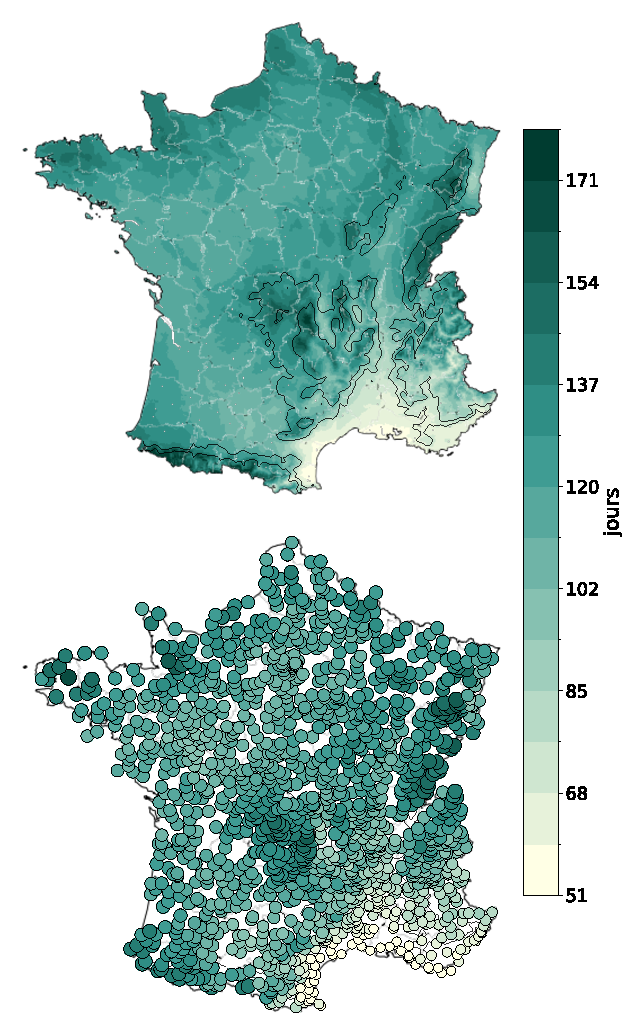
\includegraphics[keepaspectratio]{figures/jour_pluie.pdf}}
&
\pandocbounded{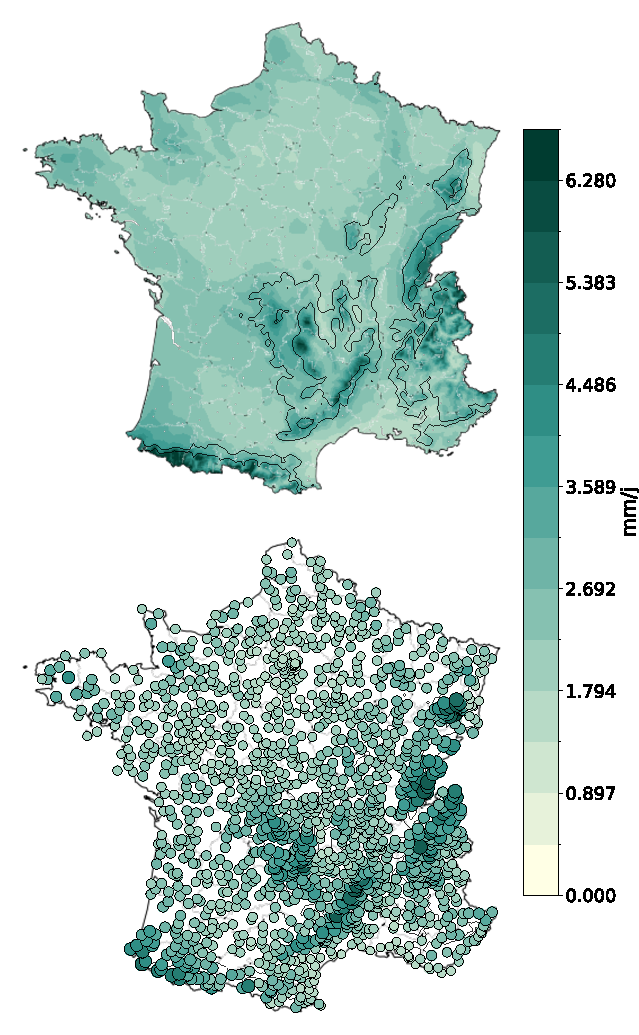
\includegraphics[keepaspectratio]{figures/mean_pluie_jour.pdf}}
&
\pandocbounded{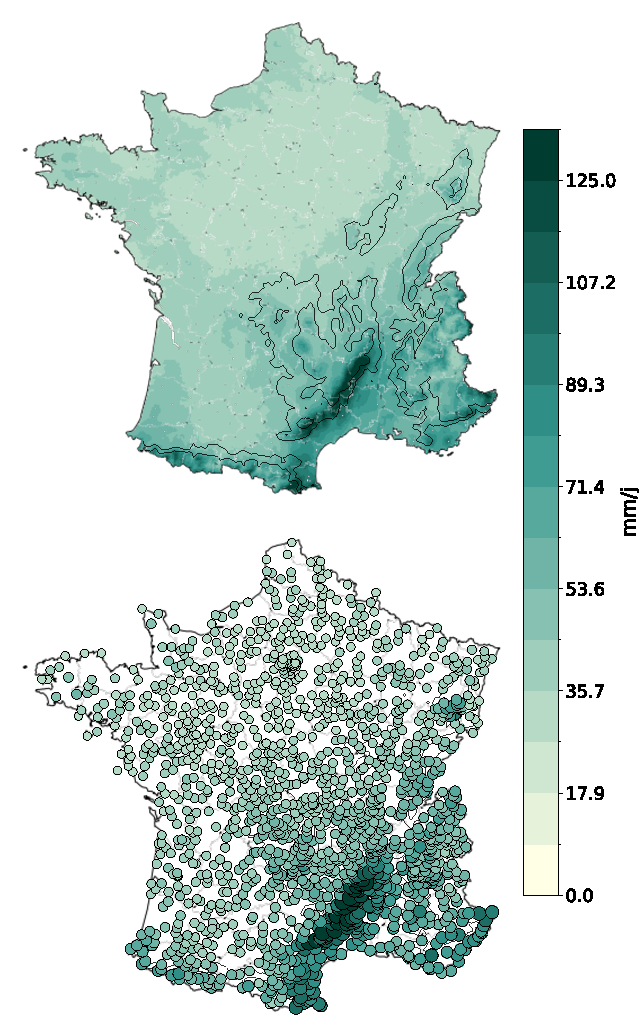
\includegraphics[keepaspectratio]{figures/mean-max_pluie_jour.pdf}} \\
\(r =\) 0.95 (n = 1583) & \(r =\) 0.94 (n = 1583) & \(r =\) 0.96 (n =
1583) \\
\end{longtable}

\begin{center}
Figure 1: Climatologie et corrélation entre le modèle AROME et les stations Météo-France issues de données journalières allant de 1959 à 2022 pour une année hydrologique.
\end{center}

\subsubsection{Corrélation entre le modèle AROME et les stations
Météo-France}\label{corruxe9lation-entre-le-moduxe8le-arome-et-les-stations-muxe9tuxe9o-france}

Quelle que soit la climatologie analysée (Figure 2), le modèle AROME
reproduit fidèlement les observations, avec une corrélation minimale de
\textbf{0,70}. Indépendamment de l'échelle temporelle
retenue\,---\,journalière (1959‑2022 ou 1990‑2022) ou horaire
(1990‑2022)\,---\,et de la saison, les champs simulés s'accordent très
bien avec les données mesurées\,: la corrélation varie entre
\textbf{0,92} et \textbf{0,98} pour le nombre de jours de pluie et le
cumul des précipitations.

Cette performance se maintient pour la moyenne des maxima journaliers
(périodes 1959‑2022 et 1990‑2022) sur l'année hydrologique, l'automne,
l'hiver et le printemps, mais elle se dégrade en été, avec une
corrélation de \textbf{0,85}. À l'échelle horaire, la qualité de
l'estimation des maxima se détériore encore\,: la corrélation baisse de
0,4 à 0,8\,point selon la saison pour l'année hydrologique, l'automne et
l'hiver, et chute à \textbf{0,70} au printemps et en été où \(ME =\)
-3.75 mm/h (-26.3\%). AROME tend donc à sous-estimer les précipitations
extrêmes estivales.

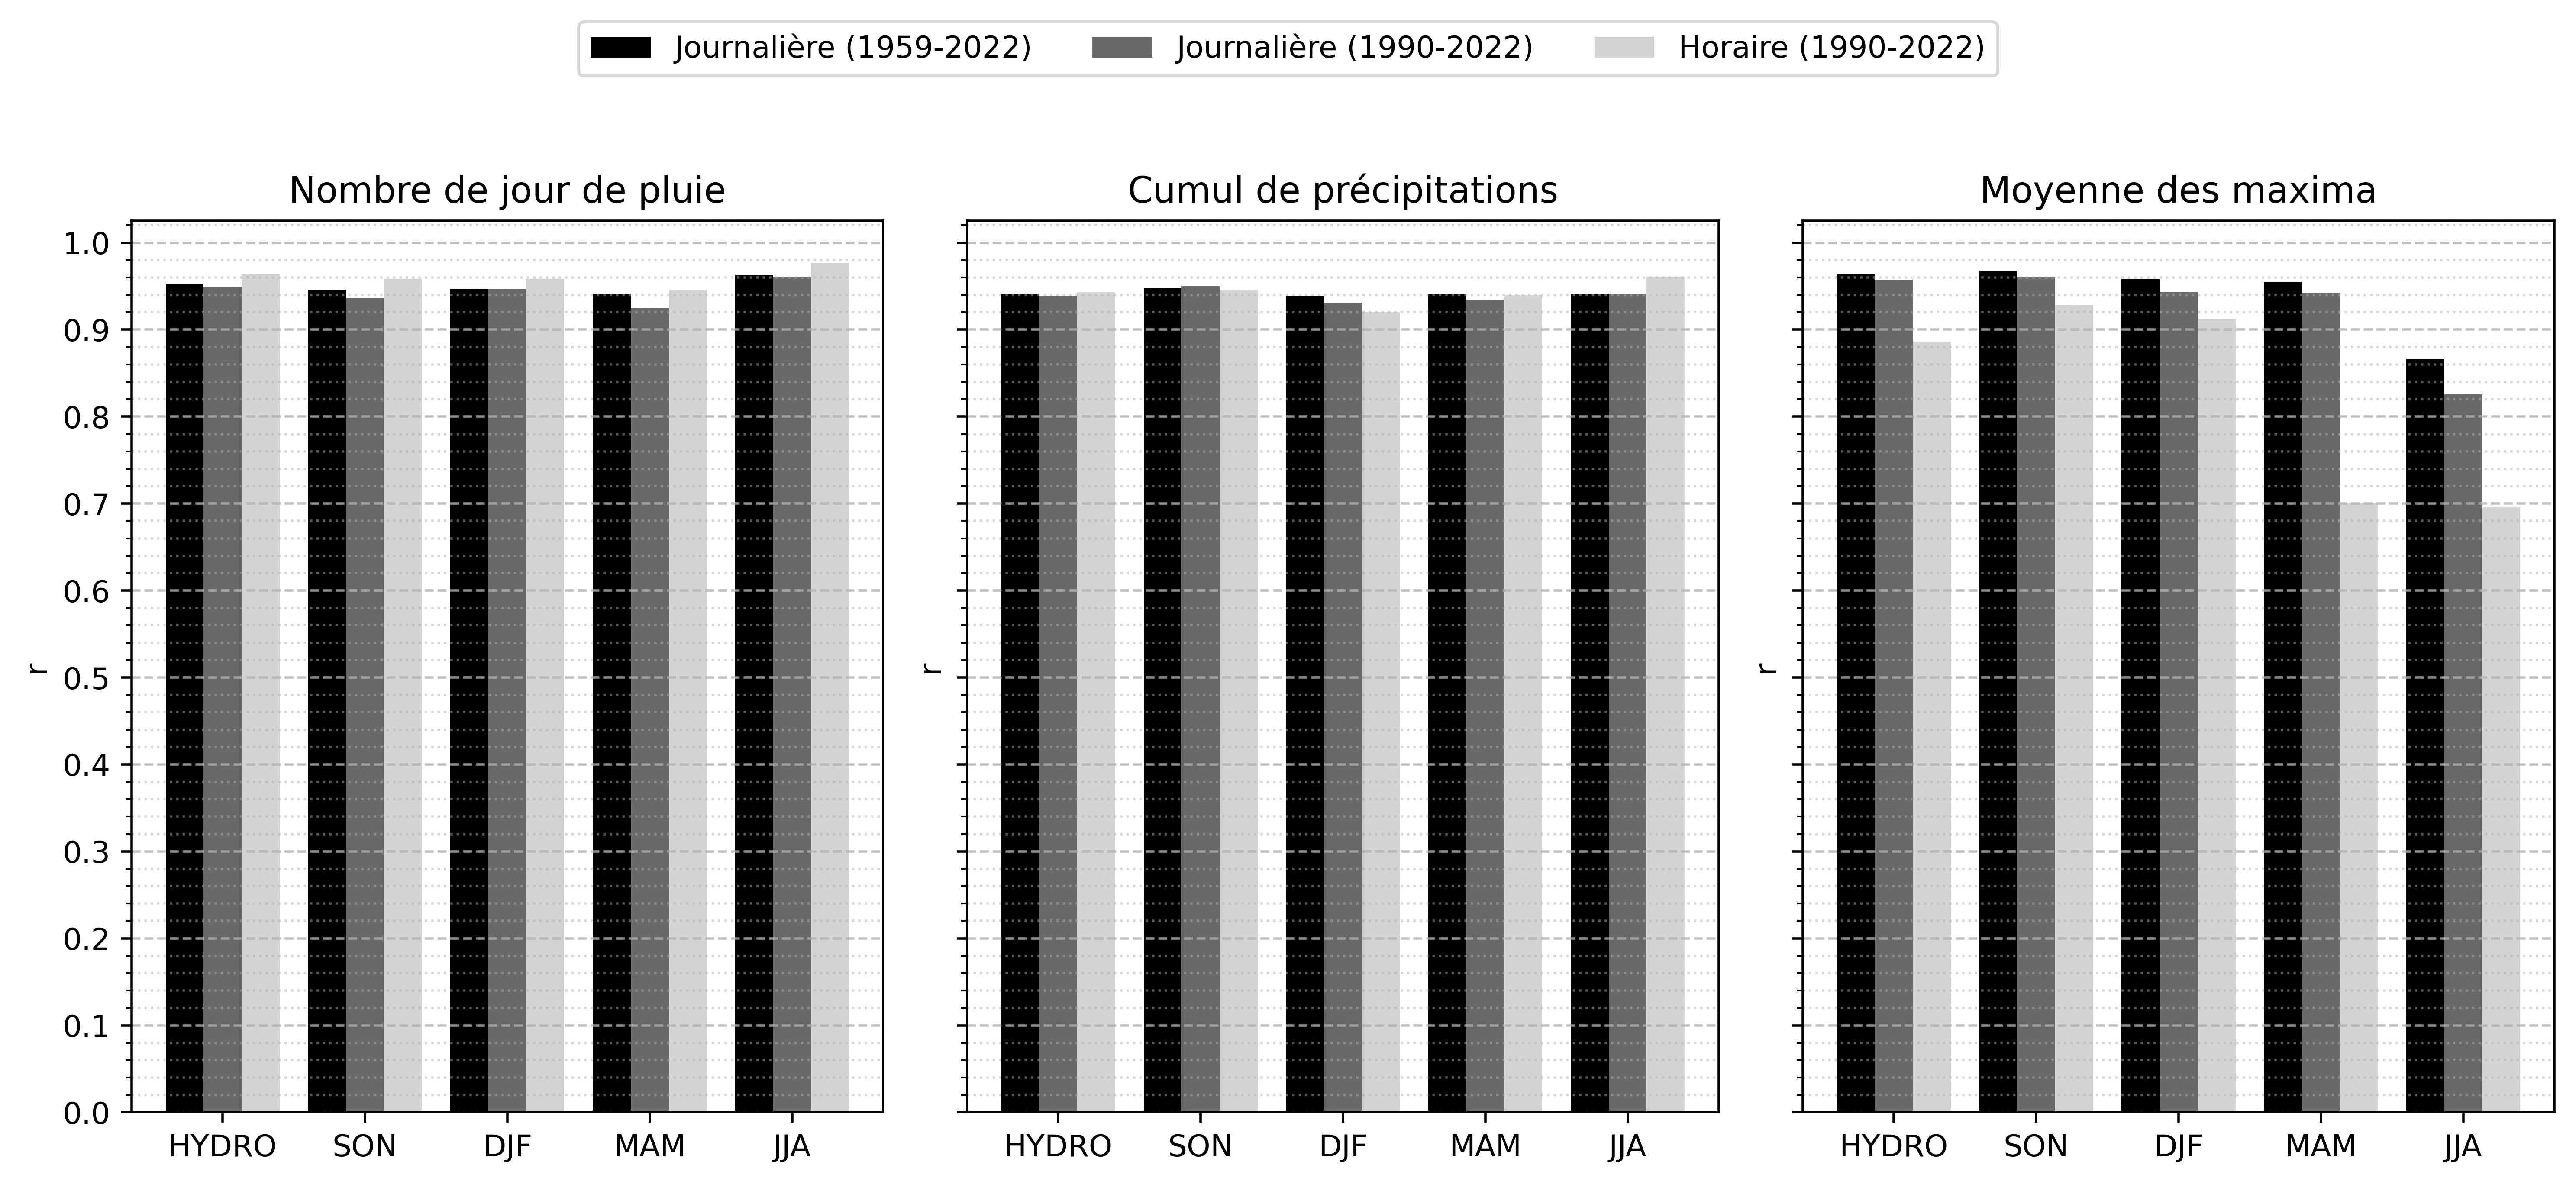
\includegraphics[width=1\linewidth,height=\textheight,keepaspectratio]{figures/histo_numday_mean_mean-max.png}

\begin{center}
Figure 2: Corrélations des données climatologiques entre le modèle AROME et les stations Météo-France pour chacune des sources de données.
\end{center}

\subsection{Evaluation des précipitations
extrêmes}\label{evaluation-des-pruxe9cipitations-extruxeames}

\subsubsection{Tendances relatives du niveau de retour 10 ans
significatif}\label{tendances-relatives-du-niveau-de-retour-10-ans-significatif}

Sur la série journalière 1959--2022 (Figure 3, panneau \textbf{J}), les
distributions mensuelles des tendances relatives s'étendent typiquement
de --50\,\% à +50\,\%, avec quelques extrêmes atteignant ±100\,\%
(juillet, août, décembre). La tendance moyenne est de -4.6\% pour AROME
et -1.6\% pour les stations. Les médianes restent proches de 0
(±10\,\%), mais s'en écartent positivement au printemps (mars--mai) et
négativement en fin d'hiver ainsi qu'en fin d'été / début d'automne
(février, mars, août, septembre). La forme des distributions est
comparable entre AROME et les stations, bien que l'étalement soit plus
marqué pour les stations. Les médianes sont presque toujours plus
élevées pour les stations que pour AROME.

Lorsque l'on restreint la période à 1990--2022 (Fig.\,4, panneau
\textbf{J}*), la dispersion relative augmente pour tous les mois (queues
positives plus longues), tandis que les médianes demeurent modérées
(±20--30\,\%). La moyenne des médianes est de -0,7\% pour AROME et 0,5\%
pour les stations. La tendance moyenne est de 2.4\% pour AROME et 3.5\%
pour les stations. Elles restent positives au printemps (mars--juin) et
en début d'hiver (octobre) (+20 à +50\,\%), et négatives en hiver
(décembre--février), ainsi qu'en août et septembre (--20 à --50\,\%).
Les distributions et leurs médianes sont alors très proches entre AROME
et les stations.

Sur les données horaires 1990--2022 (Fig.\,4, panneau \textbf{H}), la
dispersion s'accroît encore avec quelques valeurs extrêmes
\textgreater{} +400\% (tronquées sur la figure). La moyenne des médianes
est de 5,2\% pour AROME et 15,1\% pour les stations. La tendance moyenne
est de 8.5\% pour AROME et 29.1\% pour les stations. Les médianes sont
d'environ ±50\%, ponctuellement jusqu'à ±80/100\%. Elles sont positives
en début d'hiver puis en février et juin (+20 à +60\,\%), et négatives
en août et septembre (--20 à --25\,\%). La distribution est similaire
entre AROME et les stations, mais plus étalée pour ces dernières ; leurs
médianes y dépassent presque toujours celles d'AROME.

Le rapport entre les tendances moyennes (respectivement des moyennes des
médianes) \textbf{H} et \textbf{J} est de -1,8 (respect. -1,3) pour
AROME et -17,9 (respect. -12,5) pour les stations et entre \textbf{J*}
et \textbf{J} de -0.5 (respect. 0,2) pour AROME et -2.2 pour les
stations (respect. -0,4). Quel que soit le type de données (\textbf{J},
\textbf{J}* ou \textbf{H}), les distributions des tendances relatives
convergent en août et septembre, mais divergent nettement en février et
en mai. D'un mois à l'autre, les profils changent sans continuité
apparente ; une agrégation purement saisonnière ne semble donc pas
représentative de la variabilité réelle.

\includegraphics[width=1\linewidth,height=\textheight,keepaspectratio]{../outputs/boxplot/violin_signif.pdf}

\begin{center}
Figure 3: Tendances relatives significatives du niveau de retour 10 ans de 1995 à 2022 communes au modèle AROME et aux stations de Météo-France pour chacune des sources de données (\textbf{J} : données journalières 1959-2022, \textbf{J*} : données journalières 1990-2022, \textbf{H} : données horaires 1990-2022).
\end{center}

\subsubsection{Corrélation des tendances relatives entre le modèle AROME
et les stations
Météo-France}\label{corruxe9lation-des-tendances-relatives-entre-le-moduxe8le-arome-et-les-stations-muxe9tuxe9o-france}

À l'échelle quotidienne (1959‑2022), les corrélations des tendances se
situent entre \textbf{0,14} (HYDRO) et \textbf{0,23} (DJF) pour les
saisons et entre \textbf{0,07} (JUI) et \textbf{0,51} (DEC) pour les
mois, plusieurs mois atteignant ou dépassant \textbf{0,40} (JAN, MAR,
AOU, NOV) (Figure 4). Sur la période restreinte (1990‑2022), les valeurs
saisonnières couvrent \textbf{0,13--0,29} et les valeurs mensuelles
\textbf{0,02--0,47} (JAN \textbf{0,47} ; DEC \textbf{0,35}). À l'échelle
horaire (1990‑2022), les saisons présentent des corrélations faibles
comprises entre \textbf{--0,08} (MAM) et \textbf{0,05} (DJF et SON) et
les corrélations suivant les mois s'étendent de \textbf{0,02} (SEP, OCT)
à \textbf{0,42} (FEV).

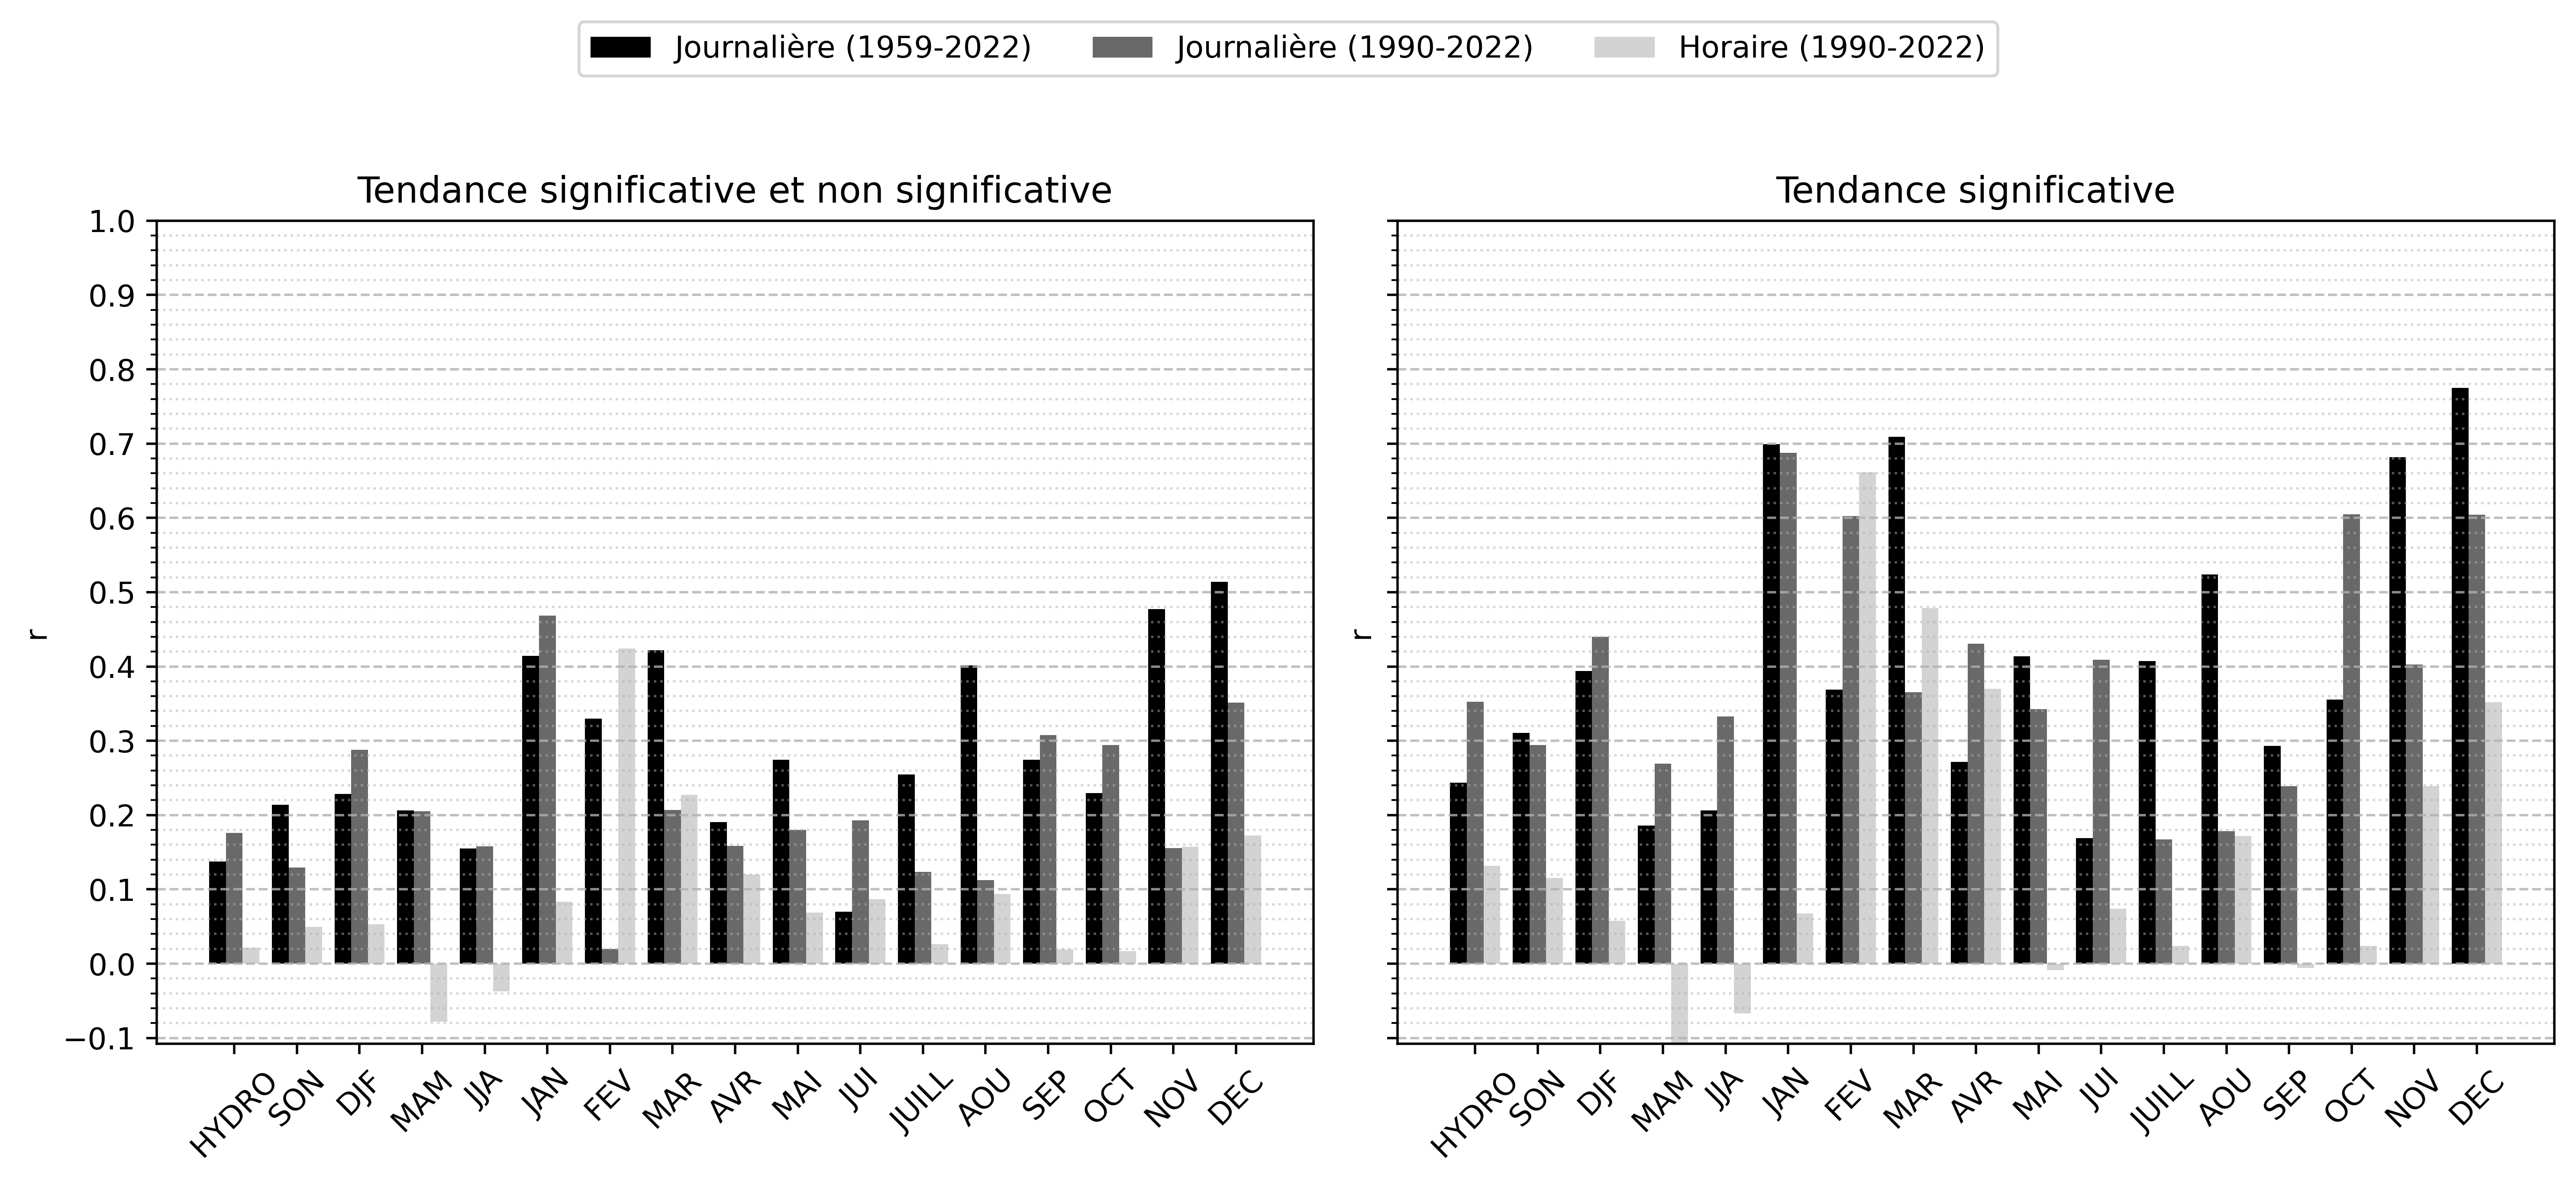
\includegraphics[width=1\linewidth,height=\textheight,keepaspectratio]{figures/histo_z_T_p.png}

\begin{center}
Figure 4: Corrélations des tendances relatives entre le modèle AROME (première ligne) et les stations Météo-France (deuxième ligne) pour chacune des sources de données.
\end{center}

En restreignant aux tendances significatives par vraisemblance profilée,
l'échelle quotidienne (1959‑2022) affiche des corrélations saisonnières
de \textbf{0,19} (MAM) à \textbf{0,39} (DJF) et des valeurs mensuelles
de \textbf{0,17} (JUI) à \textbf{0,77} (DEC), avec d'autres mois
marquant une corrélation élevée (JAN \textbf{0,70} ; MAR \textbf{0,71} ;
NOV \textbf{0,68} ; AOU \textbf{0,52}). Pour la période restreinte
(1990‑2022), les valeurs saisonnières vont de \textbf{0,27} (MAM) à
\textbf{0,44} (DJF) et les valeurs mensuelles de \textbf{0,17} (JUILL) à
\textbf{0,69} (JAN), avec des valeurs supérieures à 0,60 en février,
octobre et décembre. À l'échelle horaire (1990‑2022), les valeurs
saisonnières couvrent \textbf{--0,20--0,13} et les valeurs mensuelles
\textbf{--0,01--0,66}. La restriction aux tendances significatives
augmente fortement les corrélations quotidiennes, avec des maxima
mensuels élevés. Le gain est marqué en hiver et en fin d'été / automne
(JAN, MAR, NOV, DEC, AOU). À l'échelle horaire, même après filtrage,
l'amélioration reste partielle : quelques mois s'améliorent (FEV) mais
plusieurs périodes sont marquées par des corrélations proches de zéro ou
légèrement négatives (MAI, SEP).

\paragraph{Saisonnalité récurrente de la
performance}\label{saisonnalituxe9-ruxe9currente-de-la-performance}

L'hiver (DJF) et les mois hivernaux isolés (DEC, JAN, MAR) concentrent
les plus fortes corrélations, que ce soit sur la période longue ou
restreinte, et surtout après filtrage. Le printemps (MAM) et le début
d'été (JUI, JUILL) affichent systématiquement les valeurs les plus
basses (ou minima) dans chaque configuration. La fin d'été / automne
(AOU, NOV) fournit des corrélations intermédiaires à élevées une fois
les tendances significatives retenues.

\paragraph{Hiérarchie claire des échelles
temporelles}\label{hiuxe9rarchie-claire-des-uxe9chelles-temporelles}

L'étude journalière est systématiquement plus cohérente spatialement
pour les tendances que l'étude horaire. Le filtrage de significativité
transforme la distribution journalière (multiplication des mois
\textgreater0,60), alors qu'il ne suffit pas à hisser l'horaire à un
niveau comparable (un seul mois \textgreater0,60).

\subsubsection{Cartographie des tendances relatives du niveau de retour
10 ans
significatif}\label{cartographie-des-tendances-relatives-du-niveau-de-retour-10-ans-significatif}

En annexes, l'ensemble des cartes des tendances relatives du niveau de
retour 10 ans entre 1995 et 2022 montre une cohérence spatiale entre
AROME et les stations malgré les corrélations faibles.

\paragraph{Peu de cohérence saisonnière entre extrêmes journaliers et
horaires}\label{peu-de-cohuxe9rence-saisonniuxe8re-entre-extruxeames-journaliers-et-horaires}

L'aggrégation en saison ne semble pas montrer de patterns clairs pour
les données horaires (Annexes 2 - 4.3.1.2). Pour les données
journalières de 1959 à 2022 (Annexes 2 - 4.1.1.2), la vallée du Rhônes
est marquée par une tendance relative positive sur les données observées
pour l'année hydrologique, qu'AROME ne semble pas capter. A l'autonme
(SON), les Alpes du Nord (tendance négative ; -20/-30\%) s'opposent
fortement aux Alpes du Sud (tendance positive ; +20/30\%). En hiver
(DJF), les Alpes du Nord sont encore une fois marquée par une tendance
négative (-10/-20\%), ainsi que le Massif Central (allant jusqu'à
-30\%). Au printemps (MAM), la moitié Nord de la France semble marquée
par une tendance relative fortement postive allant jusqu'à +30\% par
endroit. Cette tendance s'accentue (+50/150\%) sur toute la façade ouest
de la France pour les données journalières restreintes à 1990-2022.
Enfin en été (JJA), le pourtour méditérannée et surtout les bassins des
Pyrénées-Orientales connaissent une forte tendance négative (-20/-40\%).

\paragraph{Une tendance relative positive dans la vallée du
Rhône}\label{une-tendance-relative-positive-dans-la-valluxe9e-du-rhuxf4ne}

Dans la vallée du Rhône (Figure 5), on observe un signal
particulièrement fort. En novembre (données journalières 1959--2022),
toute la vallée du Rhône affiche une légère à modérée hausse des niveaux
de retour, typiquement de l'ordre de +10\,\% à +30\,\%. En octobre
(données journalières 1990--2022), la vallée du Rhône connaît la plus
forte augmentation\,: les secteurs autour de Valence, Montélimar et
Avignon culminent souvent entre +80\,\% et +150\,\% de croissance des
niveaux de retour. La façade méditerranéenne du sud-est et le couloir
rhodanien-méditerranéen se trouve également impactés. En février (et en
mars, voir Annexes 2-4.3.2.2) (données horaires 1990--2022), le
renforcement est lui aussi très marqué\,: la zone alpine-drômoise voit
ses retours horaires grimper de +100\,\% à +150\,\%, traduisant un
accroissement net des épisodes de pluie très soutenue en quelques
heures. Les tendances dégagées par AROME sont plus modestes (+50/100\%).

\begin{longtable}[]{@{}
  >{\centering\arraybackslash}p{(\linewidth - 4\tabcolsep) * \real{0.3333}}
  >{\centering\arraybackslash}p{(\linewidth - 4\tabcolsep) * \real{0.3333}}
  >{\centering\arraybackslash}p{(\linewidth - 4\tabcolsep) * \real{0.3333}}@{}}
\toprule\noalign{}
\begin{minipage}[b]{\linewidth}\centering
\small Données journalière (1959-2022) en novembre
\end{minipage} & \begin{minipage}[b]{\linewidth}\centering
\small Données journalière (1990-2022) en octobre
\end{minipage} & \begin{minipage}[b]{\linewidth}\centering
\small Données horaires (1990-2022) en février
\end{minipage} \\
\midrule\noalign{}
\endhead
\bottomrule\noalign{}
\endlastfoot
\pandocbounded{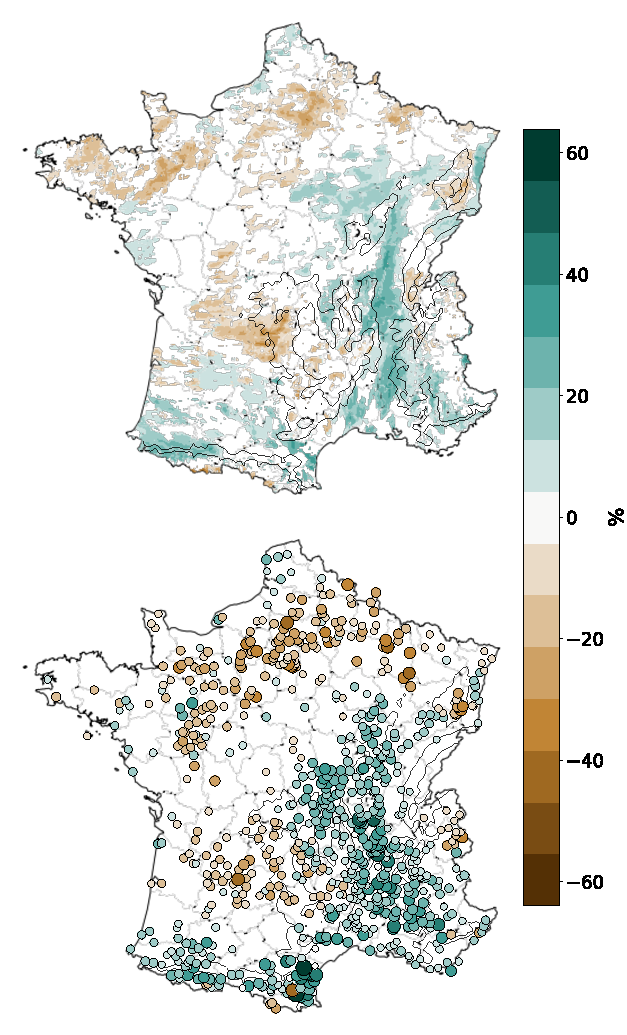
\includegraphics[keepaspectratio]{figures/jour_tot_nov.pdf}}
&
\pandocbounded{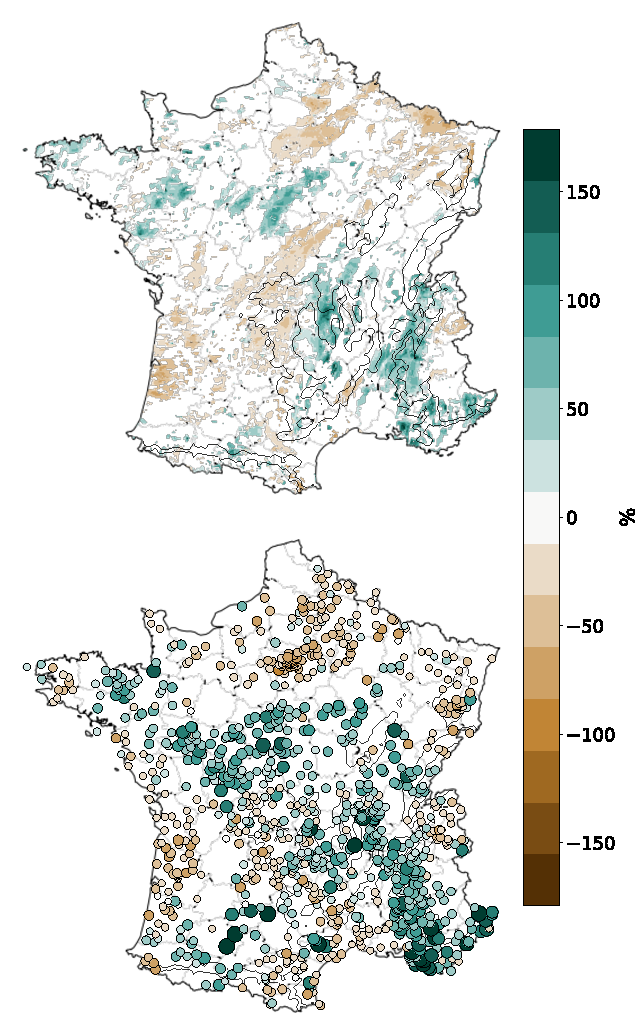
\includegraphics[keepaspectratio]{figures/jour_red_nov.pdf}}
&
\pandocbounded{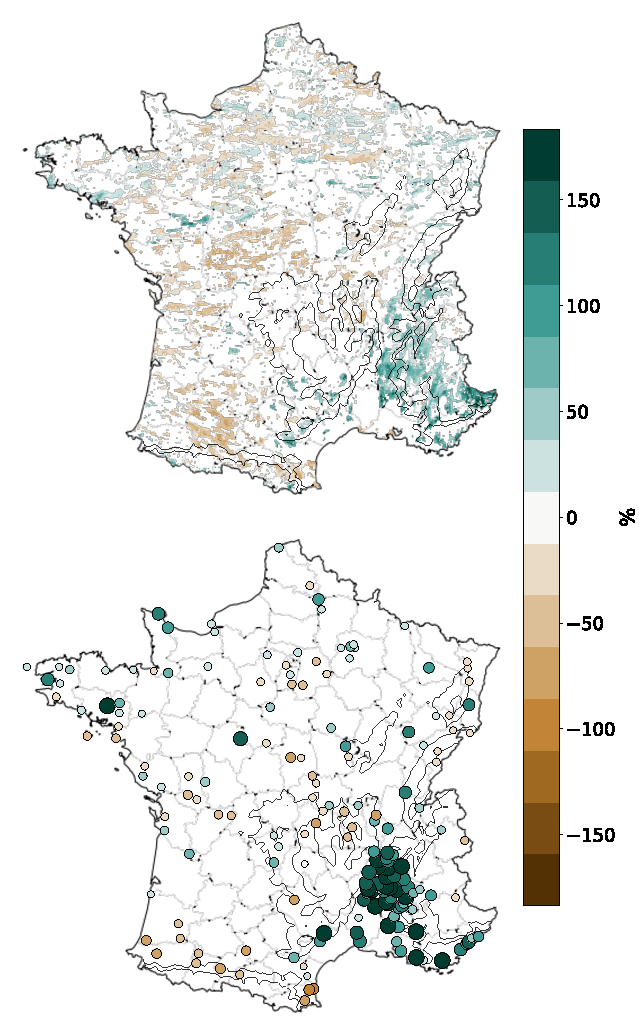
\includegraphics[keepaspectratio]{figures/horaire_nov.pdf}} \\
\(r =\) 0.68 (n = 350) & \(r =\) 0.60 (n = 346) & \(r =\) 0.66 (n =
51) \\
\end{longtable}

\begin{center}
Figure 5: Tendances relatives de 1995 à 2022 du niveau de retour 10 ans significatif entre le modèle AROME (première ligne) et les stations Météo-France (deuxième ligne) pour chacune des sources de données à différents mois (OCT, NOV, FEV). Exemple d'une station avec séries temporelles et niveaux de retour disponible en Annexe 2-6.
\end{center}

\paragraph{Une tendance relative variable des Pyrénées-Orientales à la
vallée du
Rhône}\label{une-tendance-relative-variable-des-pyruxe9nuxe9es-orientales-uxe0-la-valluxe9e-du-rhuxf4ne}

Le pourtour méditerranéen (Figure 6), en particulier le Gard, l'Hérault,
le sud Ardèche et la basse vallée du Rhône (Avignon -- Arles), présente
une forte baisse des niveaux de retour, entre -40\% à -70/80\% sur les
données journalières de la période totale en décembre. La cohérence
modèle--observation est très bonne (r = 0,77), ce qui renforce la
fiabilité de ce signal. Le signal positif persiste sur les données
tronquées (1990-2022). Les baisses restent fortes en Camargue et delta
du Rhône (jusqu'à -100 \%). En données horaires, un changement brutal
est visible. La carte montre des hausses marquées au sud du Massif
Central et jusqu'au delta du Rhône, avec des valeurs pouvant atteindre
+100\%. Les stations confirment un fort signal (allant jusqu'à +150\%)
en vallée du Rhône sud, Gard, Drôme, Ardèche. Cependant, le signal est
plus diffus et moins systématique que pour décembre. La corrélation
modèle--station chute à 0,48, ce qui traduit une variabilité horaire
plus forte et moins bien capturée. On retrouve le signal positif de
février dans la partie basse de la vallée du Rhône.

\begin{longtable}[]{@{}
  >{\centering\arraybackslash}p{(\linewidth - 4\tabcolsep) * \real{0.3333}}
  >{\centering\arraybackslash}p{(\linewidth - 4\tabcolsep) * \real{0.3333}}
  >{\centering\arraybackslash}p{(\linewidth - 4\tabcolsep) * \real{0.3333}}@{}}
\toprule\noalign{}
\begin{minipage}[b]{\linewidth}\centering
\small Données journalière (1959-2022) en décembre
\end{minipage} & \begin{minipage}[b]{\linewidth}\centering
\small Données journalière (1990-2022) en décembre
\end{minipage} & \begin{minipage}[b]{\linewidth}\centering
\small Données horaires (1990-2022) en mars
\end{minipage} \\
\midrule\noalign{}
\endhead
\bottomrule\noalign{}
\endlastfoot
\pandocbounded{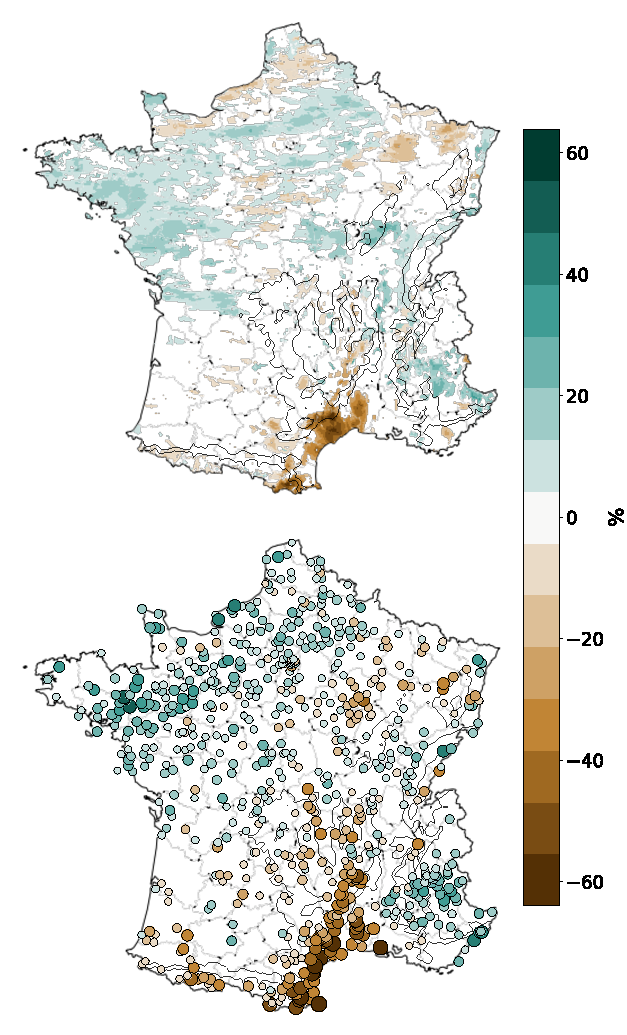
\includegraphics[keepaspectratio]{figures/jour_tot_dec.pdf}}
&
\pandocbounded{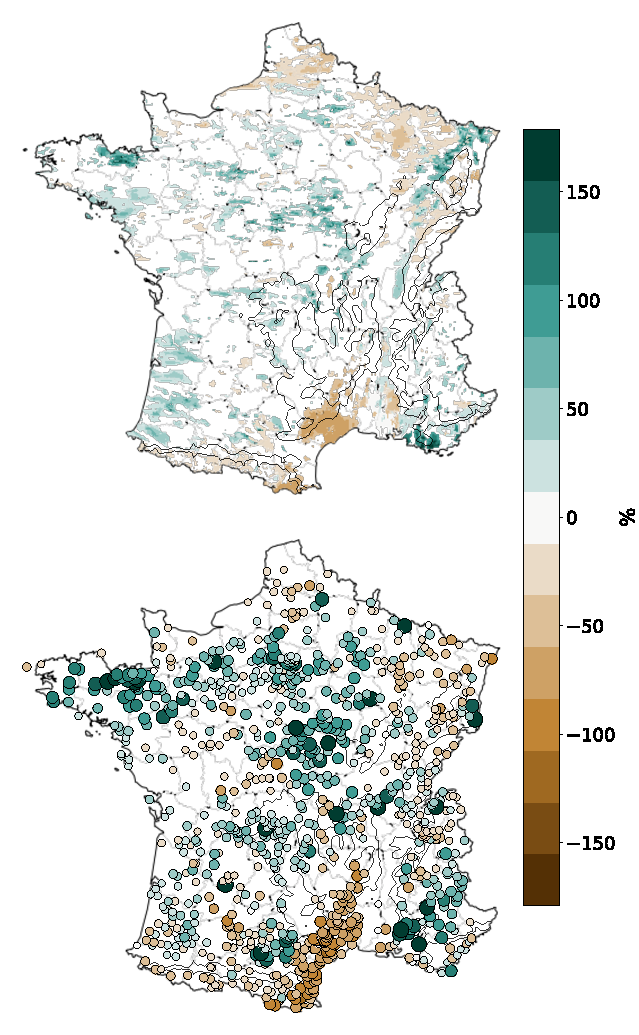
\includegraphics[keepaspectratio]{figures/jour_red_dec.pdf}}
&
\pandocbounded{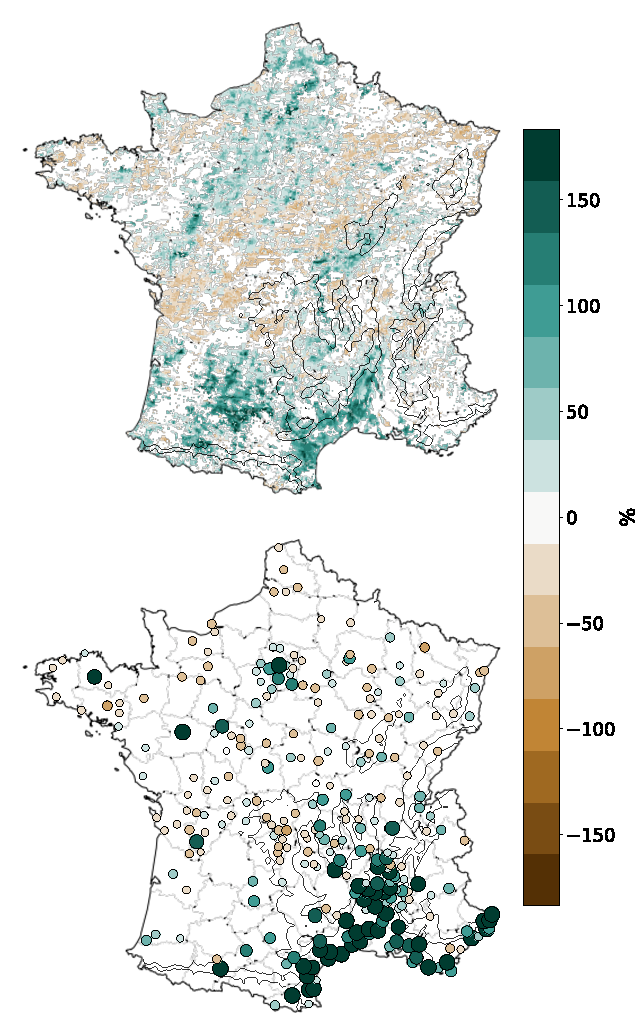
\includegraphics[keepaspectratio]{figures/horaire_mar.pdf}} \\
\(r =\) 0.77 (n = 320) & \(r =\) 0.60 (n = 316) & \(r =\) 0.48 (n =
136) \\
\end{longtable}

\begin{center}
Figure 6: Tendances relatives de 1995 à 2022 du niveau de retour 10 ans significatif entre le modèle AROME (première ligne) et les stations Météo-France (deuxième ligne) pour chacune des sources de données à différents mois (DEC, MAR).
\end{center}

\section{Discussion}\label{discussion}

\subsubsection{Fidélité spatiale de la climatologie
simulée}\label{fiduxe9lituxe9-spatiale-de-la-climatologie-simuluxe9e}

Les résultats confirment qu'AROME reproduit correctement les grands
régimes pluviométriques hexagonaux confirmé par la littérature
\citep{Fumiere2020}, \citep{caillaud2021simulation},
\citep{hess-28-2579-2024}, \citep{LucasPicher2024}. Il y a un excédent
orographique sur les Alpes, les Pyrénées et le Massif central, un
gradient atlantique‑continental marqué à l'ouest\,et un déficit
fréquentiel sur le pourtour méditerranéen. Cette cohérence avec la
réalité mesurée témoigne d'une représentation satisfaisante des forçages
dynamiques (transport d'humidité par les flux d'ouest, soulèvement
orographique, circulation de basse couche en Méditerranée).

\subsubsection{Variabilité saisonnière et représentation des
extrêmes}\label{variabilituxe9-saisonniuxe8re-et-repruxe9sentation-des-extruxeames}

La capacité d'AROME à restituer la fréquence et la quantité de
précipitations se maintient tout au long de l'année, mais la performance
chute pour la moyenne des maxima journaliers en été et davantage à
l'échelle horaire. On retrouve le fait qu'AROME sous-estime des
précipitations d'intensité élévées (\textgreater{} 40 mm/h
\citep{Caillaud2021}, \citep{poncet2024convection}) La convection
estivale reste partiellement sous‑résolue malgré la résolution spatiale
de 2,5\,km. Dans cette étude, on a pu montrer (résultats non affichés)
que la corrélation augmente lorsque la fenêtre temporelle s'agrandit à 6
ou 9h. Le modèle pourrait reproduire la cellule orageuse en\,démarrant
trop tard ou trop tôt, en étalant l'intensité sur plusieurs mailles (non
évalué par manquante de stations) ou en sous‑estimant les précipitations
maximales. Le pas de 2--3\,km est une étape majeure pour représenter la
convection sans paramétrage, mais il reste trop grossier pour certaines
applications sensibles aux maxima intenses \citep{Prein2015Review}. Il
aurait été intéressant d'introduire les données COMEPHORE (1\,km,
15\,min) de Météo-France dans cette étude mais les réanalyses ne
débutent qu'en 1997.

\subsubsection{Robustesse statistique des
signaux}\label{robustesse-statistique-des-signaux}

Une fenêtre longue (1959‑2022) réduit les incertitudes et intégre toutes
les phases climatiques en atténuant ainsi la tendance réelle\,par
mélange de plusieurs régime. Une fenêtre courte (1990‑2022) met en avant
le signal forcé récent tout en augmentant la sensiblilité aux années
extrêmes individuelles. Une archive longue est indispensable pour
quantifier la variabilité interne, mais une fenêtre centrée sur l'ère
post‑1990 est nécessaire pour capter le signal anthropique qui
s'accélère. Les deux diagnostics sont donc complémentaires\,et les
interpréter séparément évite de confondre bruit multidécoennal et
forçage à long terme.

En première approximation, les distributions mensuelles des tendances
relatives du niveau de retour 10\,ans demeurent globalement centrées
sur\,0\% entre 1959\,et\,2022. En revanche, le resserrement à 1990--2022
révèle un léger basculement vers des accroissements, particulièrement
visibles au printemps et en début d'hiver. Ce renforcement, bien que
modeste, rejoint la littérature sur l'amplification récente des
précipitations extrêmes quotidiennes en lien avec le réchauffement. Le
``dimming'', phénomène météorologique, est lié à la diminution de la
transmission du rayonnement solaire à travers l'atmosphère en raison de
la présence d'aérosols (particules fines), de polluants, ou de nuages
\citep{Wild2009_GlobalDimmingBrightening}. Entre 1950 et 1985, malgré
l'augmentation des gaz à effet de serre, il y a un refroidissement dû
aux aérosols qui a en partie ``masqué'' le réchauffement. Ce qui
explique la stagnation voire le léger refroidissement observé en France
jusque dans les années 1985. À partir des années 1985 et jusqu'en
1992\,--\,94, une fois les aérosols réduits, le réchauffement s'est
accéléré. Ainsi, une série longue (1959‑2022) échantillonne plusieurs
phases internes du climat\,: refroidissement lié au ``dimming'' puis
phase chaude des années\,1990‑2000. La variabilité multidécoennale
atténue donc la pente moyenne\,; une partie du signal récent est
noyée\,dans le bruit naturel. Une fenêtre courte centrée sur 1990‑2022
isole un régime dominé par le réchauffement rapide, la fin de la
pollution sulfatée en Europe et l'augmentation quasi linéaire du contenu
en vapeur d'eau. Le gradient thermodynamique (+7\%/°C) ressort alors
plus nettement. Si l'on impose un pas de tendance unique à\,0 (1959‑85)
puis linéaire (\textgreater\,1985) avec l'introduction d'un point de
rupture dans les modèles GEV, on compresse un virage réel de presque
10\,ans ; le modèle long absorbe cette transition, ce qui réduit la
pente moyenne par rapport au modèle court qui ne se fixe que sur la
partie linéaire. Dans la fenêtre longue, les premières années de la
pente post point de rupture englobent cette phase de rattrapage, ce qui
lisse la tendance. Ce phénomène pourrait expliquer une tendance
nationale observée de --1,6\% sur 1959‑2022 contre +3,5\% sur 1990‑2022.

Ces différences sont corroborées par un effet statistique expliqué par
\citet{DeGaetano2018} qui s'intéressent au taux relatif de changement du
paramètre de localisation \(\mu\) et qui montrent que pour des tendances
supérieures à +0,5\% par an, raccourcir la fenêtre de 60 à 30\,ans
modifie la pente estimée des niveaux de retour 10 ans de 10 à 20\%.

\subsubsection{Hiérarchie temporelle et influence de la
significativité}\label{hiuxe9rarchie-temporelle-et-influence-de-la-significativituxe9}

Le filtrage statistique élimine nombre de sites où le signal est dominé
par le bruit climatique, améliorant la cohérence spatiale des tendances
et donc les diagnostics régionaux. À l'échelle journalière, les valeurs
mensuelles des corrélations AROME--stations oscillent entre 0,40
et\,0,77 après filtrage par significativité, contre moins de\,0,20 à
l'échelle horaire. Ce saut témoigne de la difficulté d'AROME à expliquer
les maxima convectifs fins (1h).

Le découpage saisonnier met en lumière une hiérarchie marquée par
l'hiver (DJF) qui concentre systématiquement les corrélations les plus
fortes et des hausses modérées à marquées des niveaux de retour. En
hiver, les précipitations en Europe occidentale viennent des
perturbations atlantiques véhiculées par les flux d'ouest. Leur
intensité dépend directement de la quantité de vapeur d'eau dans ces
masses d'air, qui augmente avec la température selon la loi de
Clausius--Clapeyron. C'est pourquoi des hivers plus doux peuvent parfois
être aussi plus pluvieux, même avec une dynamique atmosphérique
identique. Le printemps et le début d'été (MAM--JUI) enregistrent au
contraire les minima systématiques. Cela révèle la difficulté
persistante, même à résolution 2,5 km, à représenter la\,convection
faiblement organisée typique de cette saison.\,Le réchauffement diurne
déclenche surtout des orages isolés d'origine locale. L'influence des
perturbations atlantiques diminue, car le jet‑stream et ses systèmes
frontaux se déplacent vers le nord. Le cisaillement vertical
s'affaiblit, empêchant l'organisation des orages en structures durables.
Il en résulte des précipitations brèves, très localisées et peu
structurées que le couple simulation--observations capture encore mal.
En août et septembre, la convergence relative des distributions
(médianes proches et corrélations \textless\,0,20) traduit une
variabilité élevée et une contribution partagée entre épisodes orageux
continentaux et systèmes méditerranéens précoces. La mixité des
mécanismes pluvieux réduit la cohérence entre sites et la capacité
d'AROME à reproduire la saisonnalité des tendances.

\subsubsection{Signaux régionaux contrastés~: focus sur la vallée du
Rhône et le pourtour
méditerranéen}\label{signaux-ruxe9gionaux-contrastuxe9s-focus-sur-la-valluxe9e-du-rhuxf4ne-et-le-pourtour-muxe9diterranuxe9en}

La vallée du Rhône semble être un «\,hot‑spot\,» des tendances positives
du niveau de retour, cohérent avec la recrudescence d'événements
cévenols à l'automne et de perturbations orographiques renforcées en
flux de sud \citep{Fresnay2012}. AROME sous‑diagnostique ces hausses
mais en reproduit la localisation, suggérant que la dynamique
(canalisation méridienne et levée orographique) est correctement
simulée, tandis que l'intensité convective demeure sous‑résolue.
\citet{Ribes2019} met en évidence que cette zone\,cumule le plus fort
renforcement observé sur l'ensemble du Midi méditerranéen avec un gain
d'intensité moyen de +22\% des précipitations extrêmes journalières
entre 1961 et 2015. \citet{blanchet2021explaining} montrent que, depuis
les années\,1980, l'influence méditerranéenne automnale s'est nettement
intensifiée et avancée dans la saison, avec les hausses de niveaux de
retour les plus fortes centrées sur le sillon Rhône‑Alpes et les
Cévennes. Ce «\,hot‑spot\,» est flagrant à l'échelle nationale pour les
données horaires en février. \citet{Berghald2025} montrent que les
tendances horaires hivernales sont statistiquement et spatialement
maximales sur l'axe Gard\,-\,basse vallée du Rhône, avec février comme
mois le plus contributif (+100\% sur le niveau de retour 20 ans).
\citet{Ribes2019} mettent en évidence sur la moitié sud‑est, incluant
Gard, Ardèche et Drôme, un doublement de la fréquence des
évènements\,≥\,200\,mm en 24\,h depuis\,1985\,avec la plupart associés à
des pics horaires \textgreater\,50\,mm. Depuis le début des
années\,1990, la température moyenne des mois d'hiver en France a gagné
≈+0,8°C (différence entre les normales 1961‑1990 et 1991‑2020 de
Météo‑France)\,---\,soit un pouvoir de rétention d'humidité
supplémentaire d'environ +6\% selon la relation de Clausius‑Clapeyron.
Trois leviers pourraient se cumuler en février : 1) la pluie remplace la
neige, concentrant la lame d'eau \citep{ZAQOUT2024131439} ; 2) il existe
des pentes de \textasciitilde12\%/°C pour les extrêmes horaires lorsque
T = 0--8°C --- soit presque le double des 7\% classiques
\citep{Drobinski2016} ; et 3) des flux de sud plus humides injectent
davantage de vapeur dans un couloir orographique très efficace
\citep{LorentePlazas2020}.

Les Pyrénées‑Orientales et le delta du Rhône montre en décembre, une
tendance journalière négative marquée (‑40\,à\,‑80\,\%) qui s'étend des
Corbières à la Camargue. Le signal pourrait traduire un déplacement
latitudinal des cyclogenèses hivernales. Depuis les années\,1970, on
observe un affaiblissement --\,et parfois un léger décalage vers
l'est\,-- des dépressions dites «\,Gênes‑Ligurie\,» ou «\,Baléares‑Golfe
du Lion\,». Leur fréquence et leur profondeur contrôlent directement les
totaux quotidiens d'un épisode hivernal dans les Pyrénées‑Orientales, le
Languedoc et la Camargue \citep{Trigo2000}. De plus, le réchauffement
fait disparaître les basses couches stables (tramontane froide)
\citep{ObermannHellhund2018} qui, lorsqu'elles sont surmontées d'un flux
humide de sud‑est, favorisent les pluies. À l'échelle horaire cependant,
la signature s'inverse en mars, soulignant la superposition d'événements
courts mais intenses (orages stationnaires) décrits par
\citet{Berghald2025} jusqu'au Gard et plus précoce comme dans la vallée
du Rhône \citep{blanchet2021explaining}.

\section{Conclusion}\label{conclusion}

\section*{Remerciements}\label{remerciements}
\addcontentsline{toc}{section}{Remerciements}

Je tiens à remercier Juliette Blanchet et Antoine Blanc pour
l'encadrement rigoureux, stimulant et bienveillant tout au long de ce
stage. Leurs conseils avisés, leur disponibilité constante et leurs
nombreuses remarques constructives m'ont permis d'approfondir
considérablement mes compétences scientifiques et méthodologiques.

\section*{References}\label{references}
\addcontentsline{toc}{section}{References}

\renewcommand{\bibsection}{}
\bibliography{bibliography.bib}

\newpage

\section*{Annexes 1 : formules
mathématiques}\label{annexes-1-formules-mathuxe9matiques}
\addcontentsline{toc}{section}{Annexes 1 : formules mathématiques}

\subsection*{A.1.1. Obtention de (1)}\label{a.1.1.-obtention-de-1}
\addcontentsline{toc}{subsection}{A.1.1. Obtention de (1)}

Soit la fonction de vraisemblance
\({\displaystyle {\mathcal {L}}(\theta ;x)} : {\displaystyle \theta \mapsto f(x;\theta )}\).
Alors :
\({\displaystyle \log {\mathcal {L}}(\theta ;x_{1},x_{2},\dots ,x_{n})=\sum _{i=1}^{n}\log {\mathcal {L}}(\theta ;x_{i})}\).

Pour \(1 + \xi \frac{x - \mu}{\sigma} > 0\), avec \(\sigma > 0\) :

\[
\begin{aligned}
\log \mathcal{L}(\theta)
&= \sum_{i=1}^n \left[
  -\log \sigma
  - \frac{1 + \xi}{\xi} \log\left(1 + \xi \frac{x_i - \mu}{\sigma} \right)
  - \left(1 + \xi \frac{x_i - \mu}{\sigma} \right)^{-\frac{1}{\xi}}
\right] \\
\log \mathcal{L}(\theta)
&= -n \log \sigma
- \left(1 + \frac{1}{\xi}\right) \sum_{i=1}^n \log\left(1 + \xi \frac{x_i - \mu}{\sigma} \right)
- \sum_{i=1}^n \left(1 + \xi \frac{x_i - \mu}{\sigma} \right)^{-\frac{1}{\xi}}
\end{aligned}
\]

La log-vraisemblance \(\ell(\theta) = \log \mathcal{L}(\theta)\) s'écrit
alors :

\[
\ell(\theta)=
-\sum_{i=1}^n\Bigl[
\log\sigma
+\Bigl(1+\tfrac1{\xi}\Bigr)\log (1+\xi\;\frac{x_i-\mu}{\sigma})
+(1+\xi\;\frac{x_i-\mu}{\sigma})^{-\frac{1}{\xi}}
\Bigr]
\tag{1}
\]

\subsection*{A.1.2. Obtention des
paramètres}\label{a.1.2.-obtention-des-paramuxe8tres}
\addcontentsline{toc}{subsection}{A.1.2. Obtention des paramètres}

\(\mu_1(z_{T,1})\) et \(\sigma_1(z_{T,1})\)

En développant les paramètres soumis à un effet temporel, on a :

\[
\begin{aligned}
\mu_0 + \mu_1 t &= z_{T,0} + z_{T,1} t - \dfrac{\sigma_0 + \sigma_1 t}{\xi_0} \left[ \left( -\log\left(1 - \frac{1}{T} \right) \right)^{-\xi_0} - 1 \right]\\
\mu_0+\mu_1\,t &= \Bigl[\,z_{T,0}
-\dfrac{\sigma_0}{\xi_0}\Bigl(\bigl[-\log(1-\tfrac1T)\bigr]^{-\xi_0}-1\Bigr)
\Bigr]\;+\;\Bigl[\,z_{T,1}-\dfrac{\sigma_1}{\xi_0}\Bigl(\bigl[-\log(1-\tfrac1T)\bigr]^{-\xi_0}-1\Bigr)\Bigr]\,t\\
\end{aligned}
\]

c'est-à-dire, terme à terme :

\[
\begin{aligned}
\mu_0 &\;=\; z_{T,0}
-\dfrac{\sigma_0}{\xi_0}\Bigl(\bigl[-\log(1-\tfrac1T)\bigr]^{-\xi_0}-1\Bigr),\\[0.8em]
\mu_1 &\;=\; z_{T,1}
-\dfrac{\sigma_1}{\xi_0}\Bigl(\bigl[-\log(1-\tfrac1T)\bigr]^{-\xi_0}-1\Bigr).
\end{aligned}
\]





\end{document}
